% !TEX program = xelatex
% 컴파일: xelatex main.tex; bibtex main; xelatex main.tex; xelatex main.tex
% (Overleaf 사용 시 Compiler를 XeLaTeX 로 설정)
\documentclass[11pt]{article}

\usepackage{kotex}          % 한국어
\usepackage[margin=1in]{geometry}
\usepackage{graphicx}
\usepackage{booktabs}
\usepackage{amsmath,amssymb}
\usepackage{multirow}
\usepackage{array}
\usepackage{subcaption}
\usepackage{caption}
\usepackage{float}
\usepackage[section]{placeins}   % 그림/표가 절 경계를 넘지 못하게 고정
\usepackage{tikz}
\usetikzlibrary{arrows.meta,positioning}
\usepackage[hidelinks]{hyperref}
\usepackage{cite}

% 한글 이탤릭 폰트가 없어 \emph 의 기울임이 렌더링되지 않는다(로그의 UnBatang italic 미정의).
% 국내 학술지 관행에 맞추어 강조를 굵게로 바꾼다.
\renewcommand{\emph}[1]{\textbf{#1}}

\graphicspath{{figs/}}
\captionsetup{font=small}
\renewcommand{\figurename}{그림}
\renewcommand{\tablename}{표}

% float 배치 여유를 늘려 그림/표가 설명 텍스트와 같은 페이지에 놓이도록 한다.
\renewcommand{\topfraction}{0.9}
\renewcommand{\bottomfraction}{0.7}
\renewcommand{\textfraction}{0.1}
\renewcommand{\floatpagefraction}{0.75}
\setcounter{topnumber}{2}
\setcounter{bottomnumber}{2}
\setcounter{totalnumber}{4}

\title{STT 없이 음향 특징만으로 개인정보(PII) 형식 숫자열을\\
탐지하는 경량 CNN의 타당성 연구}
\author{김현찬 \quad 박승진 \quad 강진구 \\[2pt]
\normalsize 숭실대학교 미디어학과}
% 날짜 고정: \today 를 쓰면 재컴파일 때마다 PDF 가 바뀌어 git diff 노이즈가 생긴다.
\date{2026년 8월}

\begin{document}
\maketitle

\begin{abstract}
음성 데이터에서 개인정보(Personally Identifiable Information, PII)를 탐지하는 표준 방식은
자동음성인식(Automatic Speech Recognition, ASR)으로 발화를 텍스트로 전사(Speech-to-Text,
이하 STT)한 뒤 자연어처리(Natural Language Processing, NLP)로 민감 정보를 찾는 캐스케이드
구조이다. 그러나 이 방식은 (1) 모든 발화를 전사해야 하는 비용과 지연, (2) 전사 텍스트
자체가 민감정보 유출 표면이 되는 문제, (3) 전사 오류가 후단으로 전파되는 문제를 안고 있다.
본 연구는 전사 과정을 건너뛰고, 음성 신호를 멜 스펙트로그램으로 변환한 뒤 경량
합성곱신경망(Convolutional Neural Network, CNN)이 ``PII 형식 숫자열''의 포함 여부를 직접
판별하는 접근의 \emph{타당성(feasibility)}을 통제 실험으로 검증한다.

본 연구의 중심 결과는 성능 수치가 아니라 모델이 실제로 무엇을 재는지를 특정한 것이다.
비PII 숫자열 카테고리를 하나씩 학습에서 완전히 제외하고 그 카테고리의 오탐률을 측정하면,
12자리를 4-4-4로 끊어 읽는 제품 일련번호가 $0.947\pm0.041$로 최고인 반면 10자리를 끊지 않고
읽는 주문번호는 $0.622\pm0.096$에 그친다. 최장 연속 자릿수 런이 결정 변수라면 순서가 반대여야
하므로, 모델은 PII의 그룹 형식을 쓰지 않는다. PII 의미가 없는 순수 난수 자릿수열을 같은 TTS로
합성한 통제 자극 1{,}280개에서도 같은 결론이 나온다. 판정 비율은 자릿수에 대한 시그모이드이고
반포화점은 $11.3$자리인데, 총 자릿수를 맞추고 4자리 그룹으로 끊어 읽어도 곡선이 그대로
겹친다($11.8$자리). 즉 모델이 재는 것은 그룹 구조가 아니라 자릿수 낭독의 \emph{분량}이며, 관측된
정밀도 상한은 그 결정 축 위에서의 상한이다. 이는 과제가 원리적으로 불가능하다는 뜻이 아니다.
12자리 제품 일련번호(4-4-4)와 12자리 계좌번호(3-3-6)는 자릿수 총량이 같지만 그룹 구조가
다르므로, 그룹 경계를 실제로 쓰는 모델이라면 가를 수 있다. 본 모델이 쓰지 않을 뿐이며,
따라서 이 상한은 남은 개선 여지를 가리키는 좌표이지 과제의 한계가 아니다.

이 상한 아래에서의 성능은 다음과 같다. 직접 설계한 60{,}706 파라미터 CNN은 전화번호 단일
유형의 통제 평가셋에서 $\text{F1}=0.955\pm0.010$, $\text{ROC-AUC}=0.997$로 음향 통계 기반
로지스틱 회귀(0.761 / 0.878)와 학습 가중치가 없는 온셋 연쇄 기준선(0.768 / 0.804)을
능가하였고, PII 유형을 넷으로 화자를 14명으로 늘린 조건에서는 $\text{F1}=0.859\pm0.011$,
재현율 $0.945\pm0.019$, hard-negative 오탐률 $0.329\pm0.034$였다(결정성을 고정한 시드 3회).
지름길 단서는 세 겹으로 배제하였다. 길이를 맞춘 평가셋에서 길이 기반 기준선이 우연 수준으로
붕괴하는 동안 CNN의 F1은 유지되었고($0.956$ 대 $0.955$), 길이 정렬용 캐리어 문장에 대한
조건부 오탐률은 캐리어가 있을 때 $0.372\pm0.047$, 없을 때 $0.000$으로 ``캐리어가 들리면
negative''라는 지름길을 부호가 반대로 기각한다. 일반화는 두 축에서 성립하였다. 14화자
leave-one-speaker-out(LOSO)에서 $\text{F1}=0.871\pm0.085$, $\text{ROC-AUC}=0.969\pm0.021$이며,
학습에서 완전히 제외한 세 PII 유형도 재현율 $0.89$--$0.92$로 탐지되었다.

Whisper 기반 STT+NLP 표준 경로와 동일 인스턴스에서 비교하면 실패 지점이 갈린다. 16자리
카드번호 재현율은 기본·프롬프트·빔 서치·결합의 네 디코딩 설정 모두에서 $0.802$--$0.864$인
반면 CNN은 세 시드 전부 $1.000$이어서, 긴 숫자열에 대한 전사 취약성이 설정 미조정이 아님을
확인하였다. 반대로 정밀도는 STT+NLP가 $1.000$ 대 $0.787$로 앞선다. 이 상보성을 근거로
``CNN 프리필터 $\rightarrow$ STT+NLP 확정''의 2단계 파이프라인과 그 손익분기 모형을 제시한다.

본 결과는 음성합성(Text-to-Speech, TTS)으로 만든 합성 데이터에 한정된다. 열화 실험에서
8\,kHz 협대역과 G.711 코덱은 F1을 $0.859$에서 $0.831$로 낮추는 데 그친다. 잡음의 영향은 잡음을
어느 대역에 넣는지에 좌우된다. 전화 통과대역(300--3400\,Hz)으로 제한한 잡음에서는 SNR 20\,dB까지
재현율이 $0.931$로 유지되고, 학습 데이터의 절반에 같은 열화를 섞어 재학습하면 SNR 5\,dB에서도
F1이 $0.777$로 평평해진다(증강 없으면 $0.491$). 대가는 깨끗한 조건의 F1 $0.859\to0.807$이다.
다만 같은 조건에서 STT+NLP가 $0.932$--$0.962$를 유지하므로, 잡음 구간에서 프리필터가 더 많이
잃는다는 사실은 남는다.
또한 평가의 지배적 불확실성은 학습 난수가 아니라 문장 템플릿 구성이어서, 템플릿 그룹
부트스트랩으로 잰 F1의 95\% 구간은 $[0.519, 0.960]$이다(재표집 단위가 여섯 그룹뿐이라
불확실성의 하한으로 읽어야 한다). 실통화 검증, 잡음 강건화, 운용
정밀도 개선을 남은 과제로 명시한다.
\end{abstract}

\section{서론}\label{sec:intro}

콜센터 상담, 회의 녹취, 음성 메모 등 음성 데이터에는 전화번호, 주민등록번호, 계좌번호,
카드번호와 같은 개인정보(Personally Identifiable Information, PII)가 빈번하게 포함된다.
개인정보보호 규제 준수와 데이터 최소화 원칙을 위해 이러한 민감 정보를 자동으로 탐지하고
비식별화(redaction)하려는 수요가 크다. 현재 표준적인 접근은 음성을
자동음성인식(Automatic Speech Recognition, ASR)으로 전사한 뒤 전사 텍스트에
자연어처리(Natural Language Processing, NLP) 기법인 개체명 인식(Named Entity Recognition,
NER)이나 정규식 패턴 매칭을 적용해 민감 구간을 찾고, 그 구간에 대응하는 오디오를 마스킹하는
캐스케이드 파이프라인이다~\cite{cohn2019audiodeid}. 주요 상용 서비스와 실시간 상담 시스템이
모두 이 구조를 채택하고 있다~\cite{azurepii,gouvea2023trustera}. 이하에서는 이 전사 단계를
관례에 따라 STT(Speech-to-Text)로도 부르며, ASR과 같은 뜻으로 사용한다.

이 구조는 세 지점에서 비용을 치른다. 우선 PII 포함 여부와 무관하게 모든 발화를 전사해야
하므로, 대량 녹취를 다룰수록 STT 호출 비용이 선형으로 증가한다. 본 연구에서 측정한
Whisper-large-v3~\cite{radford2023whisper}의 전사 지연은 클립당 $0.54$--$0.67$초이며(초기
청크 기반 파이프라인에서는 $0.36$초로 측정되었다), 뒤에서
제안할 경량 합성곱신경망(Convolutional Neural Network, CNN)의 추론 지연은 5초 윈도당
0.344\,ms이다(측정 조건은 \ref{sec:method}장). 다만 이 배수 자체는 운용 이득과 직결되지 않는다.
실제 절감은 프리필터가 얼마나 많은 발화를 걸러 내는지에 달려 있으므로,
\ref{sec:discuss:cost}절에서 트래픽 구성을 넣은 비용 모형으로 따로 계산한다. 여기에 더해 탐지 과정
자체가 민감 텍스트를 중간 산출물로 남긴다. 전사 텍스트는 PII를 평문으로 담게 되어 로그,
캐시, 저장소 전반에 새로운 유출 표면을 만들며, 공개된 상담 전사 데이터셋들이 배포 전에
별도의 비식별화 공정을 거쳐야 하는 이유도 여기에 있다~\cite{dao2025callcenter}. 탐지 단계에서
텍스트를 만들지 않으면, 적어도 선별에서 걸러지는 대부분의 발화에 대해서는 이 표면이
발생하지 않는다. 마지막으로, 전사 오류는 그대로 후단으로 전파된다. 본 연구의 비교 실험에서도
일반 발화의 단어오류율(Word Error Rate, WER) 중앙값이 0인 합성음 조건에서조차 숫자열
구간에서는 자릿수의 병합과 분절이 발생하여, 16자리 카드번호에 대한 STT+NLP 재현율이 0.852에
그쳤다. 전사 품질 전반이 좋더라도 오류가 하필 숫자열 구간에 집중된다는 뜻이다.

본 연구의 출발점은 다음 관찰이다. 전화번호나 계좌번호처럼 PII로 취급되는 숫자열은 낭독될 때
개별 숫자가 일정한 리듬으로 연속되고 자릿수 그룹 사이에 짧은 휴지가 놓이는, 비교적 규칙적인
시간-주파수 패턴을 만든다(그림~\ref{fig:melspec}). 본 연구는 이 패턴 가설을 검증한다.
성립한다면 ``어떤 숫자가 발화되었는가''라는 어휘 정보를 복원하지 않고도 ``숫자열이 PII의
형식을 띠는가''라는 비어휘적 패턴을 음향 표현만으로 판별할 수 있고, 전사 없이 동작하는 저비용
선별기를 캐스케이드 앞단에 배치하여 위의 세 비용을 동시에 완화할 수 있다.

이 가능성을 검증하기 위해 본 연구는 다음 다섯 가지 연구 질문(Research Question, RQ)에
답한다. 첫째, STT 없이 음향 특징만으로 PII 형식 숫자열을 탐지하는 것이 실제로 가능한가, 즉
타당성이 성립하는가(RQ1). 둘째, 그렇게 얻은 성능이 무엇에서 오는가. 발화 길이나 단순한
``숫자 존재'' 여부, 화자 지문 같은 인공 단서(artifact), 즉 과제의 본질과 무관한
지름길(shortcut) 단서~\cite{geirhos2020shortcut}를 배제한 뒤, 남는 신호가 정말 ``PII의
형식''인지 아니면 더 단순한 양인지를 \emph{측정}한다. 본 연구는 이 질문을 반박이 아니라
결정 함수의 특정으로 다룬다(RQ2). 셋째, 학습에 없던 화자와
학습에서 제외한 PII 유형으로 일반화되는가(RQ3). 넷째, 표준 경로인 STT+NLP와 비교했을 때 어떤
운용 위치가 합리적인가(RQ4). 다섯째, 이 과제에 적합한 모델 규모는 어디인가, 즉 대규모
사전학습 백본이 소형 전용 모델보다 유리한가(RQ5).

이를 위해 지름길 단서를 차단하도록 설계한 한국어 합성 음성 데이터셋을 구축하였다. 핵심
설계 결정은 두 가지다. 하나는 클래스를 가리지 않고 문장 안의 모든 숫자를 한국어 자릿수
발음으로 강제 변환하여, 두 클래스의 차이가 ``읽는 방식''이 아니라 ``숫자열 형식''만 남게 한
것이다. 다른 하나는 PII가 아닌 숫자열(날짜, 가격, 주문번호 등)을 담은 어려운 음성
표본(hard-negative)을 negative의 상당 부분으로 투입하여, ``숫자가 들린다''는 단서만으로는
과제가 풀리지 않게 한 것이다.

본 연구의 기여는 다음 여섯 가지이다. (i) STT-free 음향 PII \emph{형식} 탐지 과제를
정식화하고, 지름길 단서를 차단한 통제 데이터셋과 템플릿 누수 없는 평가 프로토콜을
설계하였다. (ii) 길이 불변, ``숫자 존재''-``형식'' 분리, 캐리어 문장의 조건부 검정이라는 세
겹의 통제 실험으로 성능이 지름길 단서로 설명되지 않음을 보이고, 나아가 \emph{모델의 결정
함수를 직접 특정}하였다. 카테고리별 미학습 오탐률과 통제 자극 실험은 결정 변수가 그룹 구조가
아니라 등간격 단음절 연쇄의 분량임을 보여 주며, 이는 현재 모델이 도달한 정밀도 상한이
어느 축 위에 놓여 있는지를 정량화한다. (iii) 화자(LOSO)와 PII 유형(held-out) 두 축의 일반화를 정량적으로
검증하였다. (iv) STT+NLP 표준 경로와 동일 조건에서, 그리고 네 가지 디코딩 설정에서 직접
비교하여 긴 숫자열에 대한 전사 취약성이 설정 미조정이 아님을 확인하고, 두 접근의 실패 지점이
상보적임을 근거로 2단계 파이프라인과 그 손익분기 모형을 제시하였다. (v) 모델별 학습률
스윕을 포함한 비교에서, 60{,}706 파라미터 경량 CNN이 각 모델에 가장 유리한 학습률을 고른
뒤에도 27.8M ImageNet 사전학습 백본을 능가함을 보였다. (vi) 협대역·코덱·잡음 열화를
실측하되 잡음을 전화 통과대역으로 제한해야 표적 도메인의 조건이 됨을 보이고, 잡음 증강 학습이
SNR 5\,dB까지 성능을 평평하게 만든다는 것과 그 대가가 깨끗한 조건의 F1 $0.05$임을 정량화하였다.

이후 논문의 구성은 다음과 같다. \ref{sec:related}장에서 관련 연구를 정리하고,
\ref{sec:data}장에서 과제 정식화와 데이터 생성 과정을, \ref{sec:method}장에서 특징 추출,
모델, 분할과 학습, 평가 프로토콜을 기술한다. \ref{sec:exp}장에서 실험 결과를 제시하고
\ref{sec:discuss}장에서 논의한 뒤, 합성 음성이라는 통제 조건에서 얻은 결과의 범위를
\ref{sec:limit}장에서 밝히고 \ref{sec:conclusion}장에서 결론을 정리한다.

\section{관련 연구}\label{sec:related}

\subsection{\texorpdfstring{ASR $\rightarrow$ NLP}{ASR-NLP} 캐스케이드 기반 음성 비식별화}
음성에서 PII를 제거하는 문제는 Cohn 등~\cite{cohn2019audiodeid}이 오디오 비식별화라는 개체명
인식 과제로 정식화하였다. 이들은 ASR로 전사한 뒤 전사 텍스트에서 개체명을 인식하고 다시
오디오 구간으로 정렬하는 세 단계 파이프라인과 그에 맞는 평가 지표를 제안했으며, 이 구조가
이후 상용 시스템의 사실상 표준이 되었다~\cite{azurepii}. Trustera~\cite{gouvea2023trustera}는
이를 실시간 상담으로 확장하여 ASR과 자연어이해 모듈, 오디오 레닥터를 파이프라인으로 연결해
상담원이 카드번호를 듣지 않도록 하면서 대화의 자연스러움을 유지한다. 대규모 상담 전사
데이터셋을 공개한 연구~\cite{dao2025callcenter}에서도 배경 잡음과 교차 발화 같은 요인이 전사
품질에 영향을 준다는 점, 그리고 공개 전에 별도의 PII 비식별화 공정이 필요하다는 점이
보고된다.

이러한 시스템들이 공통적으로 안는 구조적 취약성은 텍스트 단계가 ASR 출력에 전적으로
의존한다는 데 있다. 구어 숫자는 발화 속도와 휴지에 따라 다르게 전사되고, 하나의 번호가 여러
토큰이나 여러 발화 구간으로 분절되며, 숫자 하나가 누락되어도 형식 매칭이 실패한다. 본 연구의
\ref{sec:exp}장 실험은 이 취약성을 합성음이라는 최상 조건에서도 정량적으로 재현한다. 본
연구는 이 캐스케이드를 대체하려는 것이 아니라, 그 앞단에 전사 없이 동작하는 경량 선별기를
두어 호출량과 유출 표면을 함께 줄이는 것을 목표로 한다.

\subsection{ASR-free / 종단간 음성언어이해}\label{sec:related:slu}
본 연구와 방법론적으로 가장 가까운 계보는 음성에서 의미를 ASR 없이 직접 추론하는
종단간(end-to-end) 음성언어이해(Spoken Language Understanding, SLU) 연구이다. Serdyuk
등~\cite{serdyuk2018towards}은 전사 텍스트를 전혀 거치지 않고 음향 특징에서 곧바로 의도를
예측하는 구조가 가능함을 보였고, Lugosch 등~\cite{lugosch2019pretrain}은 ASR 과제로
사전학습한 음향 인코더를 SLU로 전이하여 적은 라벨로도 높은 정확도를 얻는 방법을 제시하였다.
Palogiannidi 등~\cite{palogiannidi2020asrfree}은 ASR 수준의 라벨이나 사전학습 모델 없이도
순환 구조와 데이터 증강만으로 경쟁력 있는 결과를 얻을 수 있음을 보였으며, Tomashenko
등~\cite{tomashenko2019recent}은 개체명 인식과 슬롯 채우기를 음성에서 직접 수행하기 위해 화자
적응, 연결주의 시간 분류(Connectionist Temporal Classification, CTC) 학습 기준의 변형, 순차적
사전학습을 제안하고 평가하였다. 최근에는 자기지도 학습된 음향 인코더에 CTC 보조 손실을
결합하여 성능을 끌어올리는 접근도 제안되었다~\cite{wang2023jointctc}. 이들 연구가 공유하는
동기는 본 연구와 상당 부분 겹친다. 전사 단계를 제거하면 ASR 오류가 후단으로 전파되지 않고,
시스템이 단순해지며, 텍스트라는 중간 표현이 만드는 병목이 사라진다. 여기에 더해 본 연구는
중간 텍스트가 생성되지 않는다는 사실 자체를 프라이버시 측면의 이득으로 명시적으로 다룬다.

그러나 문제 설정과 운용 목표에서는 네 가지 차이가 있다. 첫째, 라벨 공간이 다르다. 기존
SLU 연구의 목표는 의도(intent)나 슬롯(slot)처럼 \emph{어휘에 대응되는} 의미 범주인 반면,
본 연구의 목표는 ``PII의 형식을 갖춘 숫자열이 존재하는가''라는 비어휘적 상위 패턴이다.
어떤 숫자가 발화되었는지는 라벨과 무관하며, 오히려 같은 숫자 어휘가 두 클래스 모두에
등장한다. 둘째, 운용 목적이 다르다. 기존 연구는 최종 이해 결과의 정확도를 겨루지만, 본
연구의 모델은 뒤따르는 정밀 파이프라인의 호출량을 줄이는 \emph{프리필터}이므로, 균형
잡힌 정확도보다 고재현율과 초저지연이라는 비대칭적 운용점이 중요하다. 셋째, 평가의 초점이
다르다. 본 연구는 벤치마크 점수 경쟁이 아니라, 높은 점수가 지름길 단서에서 온 것이 아님을
보이는 통제 실험에 초점을 둔다. 넷째, 모델 규모가 다르다. 기존 종단간 SLU가 수천만에서
수억 파라미터의 사전학습 음향 인코더를 사용하는 데 반해, 본 연구는 60{,}706 파라미터의
전용 CNN을 처음부터 학습한다. 또한 PII 형식 라벨과 통제된 hard-negative를 함께 갖춘 한국어
음성 데이터는 공개된 바 없어 기존 SLU 벤치마크를 재사용할 수 없고, \ref{sec:data}장과 같은
자체 데이터 설계가 필요하다.

\subsection{키워드 스포팅과 경량 음향 분류}
멜 스펙트로그램과 소형 신경망으로 특정 어휘를 저전력에서 탐지하는 키워드 스포팅(Keyword
Spotting, KWS)은 본 연구가 사용하는 구현 기법을 공유하는 영역이다. Sainath와
Parada~\cite{sainath2015cnnkws}는 CNN이 완전연결 신경망보다 훨씬 적은 파라미터로 더 낮은
오거부율을 달성함을 보였고, Tang과 Lin~\cite{tang2018resnetkws}은 잔차 연결과 팽창
합성곱으로 소형 모델의 정확도를 끌어올렸으며, Berg 등~\cite{berg2021keyword}은 자기어텐션
기반 구조로 이를 확장하였다. 후속 연구들은 대부분 고립 단어
코퍼스~\cite{warden2018speech}에서 평가된다. 한편 대규모 오디오 분류에서는 AudioSet으로
사전학습한 CNN(Pretrained Audio Neural Networks,
PANNs)~\cite{kong2020panns}이나 스펙트로그램 트랜스포머(Audio Spectrogram Transformer,
AST)~\cite{gong2021ast}가
표준적인 표현 학습 방법으로 자리 잡았다. 이들은 범용 음향 사건 표현을 제공하지만 파라미터가
수천만 개에 달해 상시 동작하는 프리필터의 예산에는 맞지 않는다. 본 연구가 \ref{sec:exp}장에서
ImageNet 사전학습 백본을 비교군으로 삼은 것은 ``큰 사전학습 모델이 이 과제에서 유리한가''를
직접 묻기 위해서이다.

본 연구는 KWS와 적용 범위뿐 아니라 기술적 구성에서도 구분된다. 첫째, 탐지 단위가 다르다.
KWS는 고정된 어휘 목록의 각 항목에 대응하는 짧은 음향 앵커를 학습한다. 최근에는 음소열이나
예시 발화를 질의로 받는 개방 어휘 KWS도 제안되었으나, 이들 역시 질의를 어휘적
단위(음소열이나 예시 음향)로 명시해야 한다는 점은 같다. 본 연구의 탐지 대상에는 그렇게
명시할 수 있는 앵커 자체가 없으며, 판별에 쓰이는 신호는 개별 숫자의 정체가 아니라 숫자 낭독
구간의 지속 길이, 자릿수 그룹 경계에 놓이는 휴지의 배치, 반복되는 리듬 같은 시퀀스 구조이다.
둘째, 입력 길이와 집계 방식이 다르다. KWS는 1초 내외의 고정 윈도에서 프레임별 사후확률을
매끄럽게 만들어 판정하지만, 본 연구는 5초 윈도를 2.5초 간격으로 이동시키며 윈도 단위 확률의
최댓값으로 클립 점수를 정한다. 추론 시 윈도 점수를 최댓값으로 모으는 이 집계는 다중 인스턴스
학습(multiple instance learning)의 추론 규칙과 같은 형태이며, 숫자열이 윈도 경계에 걸쳐도
놓치지 않기 위해 필요하다. 셋째, 판별 난이도의 구조가 다르다. 본 연구의 positive와
hard-negative는 \emph{동일한 숫자 어휘 집합}으로 이루어져 있어, 어떤 숫자 단어가 등장했는지만
판정하는 KWS식 어휘 집합 탐지로는 두 클래스를 분리할 수 없다. 두 클래스를 가르는 정보는
어휘의 목록이 아니라 그 배열, 즉 연속 자릿수의 길이와 그룹 경계에 있다. 넷째, 학습 데이터의
성격이 다르다. 고립 단어가 아니라 캐리어 문장에 삽입된 연속 발화를 사용하며, 문장 템플릿이
분할 간에 겹치지 않도록 통제한다. 요컨대 본 과제는 ``무엇이 들렸는가''가 아니라 ``들린
숫자들이 어떤 구조로 배열되었는가''를 묻는 문제이며, 그 때문에 KWS에서 표준인 어휘 단위
사후확률 설계 대신 윈도 최댓값 집계와 hard-negative 통제가 요구된다.

\subsection{음성 콘텐츠 프라이버시}
음성 프라이버시 연구는 화자 신원 은닉에서 출발하여 최근에는 발화 내용 자체의 보호로
확장되고 있다. 화자 신원을 지우는 익명화가 ``누가 말했는가''를 다루는 문제라면, 본 연구가
속한 콘텐츠 프라이버시는 ``무엇을 말했는가'' 가운데 민감한 부분을 골라내는 문제이며, 두 축은
보호 대상이 서로 직교하여 실제 운용에서는 함께 적용될 수 있다. Williams
등~\cite{williams2022content}은 음성이 단어와 의미뿐 아니라 문체, 병리적 특징, 억양, 감정까지
드러낸다는 점에서 콘텐츠 프라이버시가 별도의 과제임을 지적하고, 상용 솔루션이 이용자에게
충분한 프라이버시 선택지를 제공하지 못하고 있음을 논한다. Preech~\cite{ahmed2020preech}는
전사 파이프라인 자체를 프라이버시 보존적으로 재구성하여, 음성을 분절·치환한 뒤 외부
전사 서비스에 보내고 결과를 복원함으로써 화자 특성과 텍스트 내용을 동시에 보호한다.
본 연구는 이들과 보호 지점이 다르다. Preech가 ``전사를 하되 안전하게 하는'' 접근이라면,
본 연구는 ``대부분의 발화에 대해 전사 자체를 하지 않는'' 접근으로, 탐지 단계에서 이진
신호만 산출하여 민감 텍스트가 생성되는 사건 수를 줄인다. 두 접근은 배타적이지 않으며,
프리필터를 통과한 소수의 발화에 프라이버시 보존 전사를 적용하는 결합도 가능하다.

\subsection{연구 공백과 본 연구의 위치}
표~\ref{tab:related}의 네 축을 함께 놓고 보면 본 연구의 위치가 드러난다. 본 연구는 텍스트를
생성하지 않는다는 점에서 종단간 SLU 및 KWS와 같은 쪽에 서지만, 라벨이 어휘가 아닌
\emph{형식}이라는 점에서 두 계보 모두와 갈라진다. 또한 성능 수치 자체보다 그 수치가 지름길
단서에서 오지 않았음을 보이는 통제와, 화자·PII 유형 두 축의 일반화 검증에 지면을 배분한다는
점에서 벤치마크 경쟁형 연구와 목적이 다르다. 본 연구는 이 위치에서 표준 경로와 직접 비교하여,
제안 접근이 대체재가 아니라 보완재임을 밝힌다.

\begin{table}[!htbp]
\centering
\caption{선행 연구와 본 연구의 위치 비교. ``단서 통제 검증''은 높은 성능이 과제와 무관한
지름길 단서에서 오지 않았음을 별도 실험으로 확인했는지를 뜻한다.}
\label{tab:related}
\footnotesize
\setlength{\tabcolsep}{3.5pt}
\begin{tabular}{lcccc}
\toprule
접근 & 중간 텍스트 & 라벨 공간 & 운용 목적 & 단서 통제 검증 \\
\midrule
캐스케이드 비식별화~\cite{cohn2019audiodeid,azurepii,gouvea2023trustera} & 생성함 & 어휘/개체명 & 정밀 확정 & 해당 없음 \\
종단간 SLU~\cite{serdyuk2018towards,lugosch2019pretrain,palogiannidi2020asrfree,tomashenko2019recent,wang2023jointctc} & 생성 안 함 & 의도·슬롯(어휘 대응) & 최종 이해 & 보고 안 함 \\
키워드 스포팅~\cite{sainath2015cnnkws,tang2018resnetkws,berg2021keyword} & 생성 안 함 & 고정 어휘 & 상시 대기 트리거 & 보고 안 함 \\
프라이버시 보존 전사~\cite{ahmed2020preech} & 생성함(보호) & 텍스트 전체 & 안전한 전사 & 해당 없음 \\
\textbf{본 연구} & \textbf{생성 안 함} & \textbf{숫자열 형식(비어휘)} & \textbf{프리필터} & \textbf{길이·숫자존재·캐리어(실험)} \\
\bottomrule
\end{tabular}
\end{table}

\section{과제 정식화 및 데이터셋}\label{sec:data}

\subsection{과제 정의}
입력은 5초 음향 윈도의 로그 멜 스펙트로그램 $\mathbf{X}\in\mathbb{R}^{64\times157}$이며(멜
채널 64, hop 512 표본에서 유도되는 프레임 수 157), 모델은 윈도가 PII 형식 숫자열을 포함할
확률 $f(\mathbf{X})=\mathrm{softmax}(g(\mathbf{X}))_1\in[0,1]$을 출력한다. 여기서 $g$는
2차원 로짓을 내는 신경망이다. 클립 $c$에 대해 $W(c)$는 그 클립을 2.5초 간격의 sliding
window로 덮어 얻은 5초 윈도들의 집합이며(클립이 5초보다 짧으면 저진폭 노이즈로 패딩한 윈도
한 개), 클립 점수는 $s(c)=\max_{\mathbf{X}\in W(c)} f(\mathbf{X})$로 정의한다. 최종 판정은
임계값 $\tau$에 대해 $\hat{y}(c)=\mathbb{1}[s(c)\ge\tau]$이며, 별도로 밝히지 않는 한
$\tau=0.5$를 사용한다. 프리필터 관점에서 $\Pr[s(c)\ge\tau]$는 뒤따르는 STT 단계로 넘어가는
클립의 비율, 즉 STT 호출률에 해당한다.

Positive는 전화번호, 주민등록번호, 계좌번호, 카드번호를 포함한 발화이고, negative는 PII가
아닌 숫자열을 포함한 hard-negative와 숫자열이 핵심 정보가 아닌 일반 발화 easy-negative로
구성한다. 본 과제는 ``문맥상 실제로 민감한가''를 판단하는 것이 아니라 ``PII 형식 숫자열이
음향적으로 존재하는가''를 판별하는 것으로 한정한다. 따라서 ``이건 예시 번호입니다''처럼
문맥상 실제 PII가 아니더라도 형식이 들리면 positive로 라벨링하며, v1 데이터셋은 이런 문맥
변형 positive를 전체의 20\%로 포함한다. 문맥 판단은 \ref{sec:exp}장에서 비교하는 STT+NLP
단계의 역할이며, 본 모델은 그 앞단의 형식 선별기이다.

\subsection{데이터 생성 파이프라인}\label{sec:data:pipeline}
PII가 포함된 실제 음성은 정의상 수집·공개가 불가능하므로, 본 연구는 통제 가능한 합성
음성 데이터셋을 직접 구축하였다. 생성은 그림~\ref{fig:pipeline}과 같이 네 단계로
이루어진다. 이하의 사양은 v2를 기준으로 서술하고, v1과 다른 점은 각 단계 끝에 밝힌다.

\begin{figure}[!htbp]
\centering
\begin{tikzpicture}[
  box/.style={draw, rounded corners=2pt, align=center, font=\small,
              minimum height=11mm, inner sep=3pt, text width=23mm},
  ex/.style={align=center, font=\scriptsize, text width=27mm},
  bk/.style={draw, dashed, rounded corners=2pt, align=center,
             font=\scriptsize, text width=32mm, inner sep=3pt},
  arr/.style={-{Latex[length=2mm]}, thick}
]
\node[box] (s1) {문장 템플릿\\+ PII 값 생성};
\node[box, right=5mm of s1] (s2) {캐리어 문장\\결합 (85\%)};
\node[box, right=5mm of s2] (s3) {숫자 표기\\정규화};
\node[box, right=5mm of s3] (s4) {TTS 합성};
\node[box, right=5mm of s4] (s5) {후처리\\16\,kHz mono};
\draw[arr] (s1)--(s2); \draw[arr] (s2)--(s3); \draw[arr] (s3)--(s4); \draw[arr] (s4)--(s5);

\node[ex, below=4mm of s1] (e1) {``제 전화번호는 \{v\}입니다.''\\ $v=$ 010-1824-0409};
\node[ex, below=4mm of s3] (e3) {010-1824-0409\\$\rightarrow$ ``공일공 일팔이사 공사공구''};
\node[ex, below=4mm of s5] (e5) {wav\,+\,metadata\\(라벨·화자·템플릿·길이)};

\node[bk, below=13mm of s4] (bk) {v1: edge-tts 3화자\\
v2: VoiceDesign \mbox{참조 1개}\\$\rightarrow$ Base 클론, 14화자};
\draw[dashed] (s4) -- (bk);
\end{tikzpicture}
\caption{데이터 생성 파이프라인. 문장 템플릿에 형식만 유효한 난수 PII 값을 삽입하고,
hard-negative에는 캐리어 문장을 결합해 positive와 길이 분포를 맞춘 뒤, 모든 숫자를 한국어
자릿수 발음으로 정규화하여 TTS로 합성한다. v2에서는 VoiceDesign으로 만든 화자별 참조 음성
1개를 Base 모델이 복제하여 14명의 일관된 합성 화자를 얻는다.}
\label{fig:pipeline}
\end{figure}

\paragraph{(1) 문장과 값 생성.}
PII 유형별로 문장 템플릿을 두고(전화 5종, 주민 4종, 계좌 4종, 카드 3종), 각 발화마다
형식만 유효한 난수 값을 생성하여 삽입한다. 전화번호는 \texttt{010-XXXX-XXXX}(11자리),
주민등록번호는 \texttt{YYMMDD-Gxxxxxx}(13자리), 계좌번호는 \texttt{3-3-6}(11--12자리),
카드번호는 \texttt{4-4-4-4}(16자리) 형식이다. 값은 난수이므로 실재하는 번호가 아니다.
hard-negative는 날짜, 주문번호(9--11자리), 송장번호(4+4자리), 가격, 우편번호(5자리),
좌석번호, 제품 일련번호(4+4+4자리), 생일, 버스번호, 수 세기의 10개 카테고리 생성기로
만들며, 우연히 전화번호 형식이 만들어지면 정규식으로 검출해 재생성한다. easy-negative는
숫자를 포함하지 않는 12종의 일반 문장이다.

v1은 전화번호 단일 유형만 다루므로 구성이 다르다. v1의 positive는 숫자열을 문장 앞·중간·끝에
배치한 일반 템플릿 10종과, ``{\{}v{\}} 형식은 예시입니다''처럼 문맥상 실제 PII가 아니지만
형식은 들리는 문맥 변형 템플릿 4종(전체의 20\%)으로 이루어진다. v1의 hard-negative
카테고리는 날짜, 주문번호, 송장번호, 호실, 창구번호, 버스번호, 가격, 수량, 우편번호, 수
세기의 10종으로 v2와 일부 다르며, 카드번호와 충돌하도록 설계한 제품 일련번호와 좌석번호는
PII 유형을 확장한 v2에서 추가되었다.

\paragraph{(2) 캐리어 문장 결합과 길이 정렬.}
hard-negative의 핵심 문장은 positive보다 짧아, 그대로 두면 클립 길이가 클래스 단서가 된다.
이를 막기 위해 hard-negative에는 85\% 확률로 ``안내 말씀드립니다'', ``확인 부탁드립니다''
같은 숫자 없는 안내 문구를 앞이나 뒤에 결합하였다. 실제로 v2 hard-negative의 길이 중앙값은
캐리어가 붙은 경우 4.72초, 붙지 않은 경우 3.04초로, 캐리어가 positive의 4.56초에 길이를
맞추는 역할을 한다. positive에는 캐리어를 붙이지 않는 대신, 숫자열이 문장 앞·중간·끝에
오도록 설계한 여러 템플릿을 사용하여 발화 내 절대 위치가 단서가 되지 않게 하였다.

캐리어가 hard-negative 쪽에 치우쳐 나타나므로(v2 기준 hard-negative의 87.1\%, positive와
easy-negative는 0\%) 모델이 ``캐리어가 들리면 negative''라는 지름길을 쓸 가능성을 검토해야
한다. 클립별 점수를 보존하여 캐리어 유무로 나눈 조건부 오탐률을 직접 측정하였고, 그 결과
이 지름길 가설은 \emph{부호가 반대}로 기각된다(\ref{sec:exp}장 표~\ref{tab:carrier}).
같은 대비는 평가 분할에 남은 세 카테고리 안에서도 예외 없이 성립한다(생일 $0.183$ 대
$0.000$, 수 세기 $0.512$ 대 $0.000$, 송장번호 $0.474$ 대 $0.000$).

다만 이 측정은 캐리어 지름길을 기각하는 대신 다른 잔여 단서를 드러낸다. 캐리어가 붙은 클립은
길이 중앙값이 4.2--5.3초로 붙지 않은 클립의 2.4--3.8초보다 길고, hard-negative 내부에서 클립
길이와 모델 점수의 스피어만 상관이 $0.482$로 총 자릿수와의 상관 $0.134$보다 크다. 5초 윈도보다
짧은 클립은 저진폭 노이즈로 채워지므로 무음 길이가 노출되지는 않지만, 윈도 안에서 \emph{음성이
차지하는 비율} 자체는 여전히 클립 길이의 함수로 남는다. 즉 \ref{sec:data:control}절의 노이즈
패딩은 길이 단서를 완전히 제거하지 못한다. 클래스 수준에서는 positive 4.56초와 hard-negative
4.64초로 길이가 맞추어져 있어 이 잔여 단서가 두 클래스를 가르지는 않으며(\ref{sec:exp}장의
length-matched 평가에서도 성능이 유지된다), 영향은 hard-negative 내부의 점수 서열에 나타난다.
이 confound 자체를 없애기 위해 캐리어를 positive에도 동일 확률로 부여한 데이터셋(v3)을
별도로 합성하여 \ref{sec:exp}장에서 재검증한다. 그 결과는 캐리어 얽힘을 없애면 분리가 오히려
뚜렷해진다는 것과, 다만 그 조작이 클래스 간 길이 정렬을 깨뜨려 두 데이터셋을 직접 비교할 수는
없다는 것을 함께 보인다.


\paragraph{(3) 숫자 표기 정규화.}
문장에 남아 있는 모든 아라비아 숫자를 한국어 자릿수 발음으로 치환한다(0$\rightarrow$공,
1$\rightarrow$일, $\ldots$). 구분자로 나뉜 그룹은 그룹 단위로 묶어 공백으로 이어 붙인다.
이 단계의 목적은 \ref{sec:data:control}절에서 상술한다.

\paragraph{(4) 음성 합성과 후처리.}
버전 1(v1)은 음성합성(Text-to-Speech, TTS) 도구인 edge-tts의 한국어 신경망 음성
3종(남성 2, 여성 1)으로, 버전 2(v2)는
Qwen3-TTS~\cite{hu2026qwen3tts} 기반의 14화자 음성 은행(\ref{sec:data:voicebank}절)으로
합성한다. v2에서는 화자를 발화 순서에 따라 균등 순환 배정하여 클래스와 화자가 상관되지 않게
하였고(화자별 128--131개), v1에서는 발화마다 세 화자 중 하나를 균등 확률로 무작위
추출하였다(화자별 655--680개). 모든 출력은 16\,kHz 모노 PCM16으로 통일하고, 파일별로 텍스트,
값, PII 유형, 화자, 템플릿 식별자, 라벨, 길이를 메타데이터로 기록한다. 생성 난수 시드는
42로 고정하였다(v1 hard-negative만 43).

\begin{table}[!htbp]
\centering
\caption{클래스별 생성 문장 예시(템플릿과 값 생성 규칙에 따라 재구성). 원문의 모든 숫자가
자릿수 발음으로 변환되어, 두 클래스가 낭독 방식이 아니라 숫자열 형식에서만 달라진다.}
\label{tab:examples}
\small
\begin{tabular}{>{\raggedright\arraybackslash}p{18mm}p{52mm}p{55mm}c}
\toprule
클래스 & 원문 & 합성에 사용된 텍스트 & 라벨 \\
\midrule
positive (전화) & 제 전화번호는 010-1824-0409입니다. & 제 전화번호는 공일공 일팔이사 공사공구입니다. & 1 \\
positive (카드) & 카드번호는 4921-3387-0155-2860입니다. & 카드번호는 사구이일 삼삼팔칠 공일오오 이팔육공입니다. & 1 \\
hard-neg (날짜) & 오늘은 2026년 3월 25일입니다. & 오늘은 이공이육년 삼월 이오일입니다. & 0 \\
hard-neg (주문) & 주문번호는 47032918665입니다. & 주문번호는 사칠공삼이구일팔육육오입니다. & 0 \\
easy-neg & 커피 한잔하면서 잠깐 쉬었다 가시죠. & (동일) & 0 \\
\bottomrule
\end{tabular}
\end{table}

\subsection{지름길 단서를 차단하기 위한 통제}\label{sec:data:control}
합성 데이터는 통제가 쉬운 대신, 설계를 잘못하면 모델이 과제의 본질과 무관한 지름길
단서로 높은 점수를 얻기 쉽다~\cite{geirhos2020shortcut}. 길이 단서에 대한 통제는
\ref{sec:data:pipeline}절의 캐리어 결합에서 이미 다루었고, 이 절에서는 나머지 세 가지를
기술한다.

\paragraph{읽기 방식 통제.}
한국어에서 숫자는 두 가지 방식으로 낭독된다. 하나는 자릿수를 하나씩 읽는 방식(``공일공
일이삼사'')이고, 다른 하나는 수량으로 읽는 방식(``삼만 오천 원'', ``이천이십육 년'')이다.
자연스럽게 문장을 합성하면 전화번호와 계좌번호는 자릿수 읽기로, 가격과 날짜는 수량 읽기로
낭독되어 두 클래스의 음소 구성과 운율이 체계적으로 달라진다. 이 상태로 학습하면 모델은
``PII 형식인가''가 아니라 ``자릿수 읽기인가''라는 훨씬 쉬운 지름길 단서만으로 두 클래스를
분리할 수 있고, 그렇게 얻은 높은 정확도는 본 연구의 주장을 전혀 뒷받침하지 못한다. 이를
막기 위해 positive와 negative를 가리지 않고 문장 안의 \emph{모든} 숫자를 자릿수 발음으로
강제 변환하였다. 예컨대 hard-negative의 원문 ``오늘은 2026년 3월 25일입니다''는 ``오늘은
이공이육년 삼월 이오일입니다''로 합성된다(표~\ref{tab:examples}). 그 결과 두 클래스는
사용하는 음소 목록과 낭독 스타일이 사실상 동일해지고, 남는 차이는 오직 숫자열의 형식, 즉
연속되는 자릿수의 길이와 그룹 경계의 배치뿐이다. 다만 hard-negative의 ``수 세기''(``하나 둘
셋 넷 다섯 여섯 일곱'')는 아라비아 숫자를 포함하지 않아 자릿수 변환의 대상이 아니며, 자릿수
낭독이 아닌 고유어 수사가 연속될 때에도 오탐이 발생하는지를 보기 위한 별도 조건으로
포함하였다.

\paragraph{hard-negative 설계.}
negative가 숫자를 포함하지 않는 일반 발화뿐이라면, ``숫자 소리가 들리는가''라는 단일
규칙만으로도 높은 정확도가 나온다. 이 경우에도 타당성 주장은 성립하지 않는다. 따라서
숫자를 포함하되 PII가 아닌 발화를 negative의 상당 부분으로 투입하였다. 특히 v2에서는
주문번호를 9--11자리, 제품 일련번호를 4+4+4자리로 설계하여 각각 계좌·전화번호, 카드번호와
자릿수 길이 및 그룹 구조가 의도적으로 충돌하도록 만들었다. 이들 hard-negative는 앞의 읽기
방식 통제에 따라 positive와 동일하게 자릿수로 낭독되므로, ``숫자 존재''라는 단서는 두 클래스
사이에서 상수가 된다. 결과적으로 hard-negative에 대한 오탐률(False Positive Rate, FPR)은
모델이 숫자의 유무를 넘어 무엇을 재고 있는지를 직접 측정하는 지표가 된다. 형식적으로 이
지표는 $\frac{1}{|H|}\sum_{c\in H}\mathbb{1}[s(c)\ge\tau]$로 정의하며 $H$는 평가셋의
hard-negative 클립 집합이다. 분모가 negative 전체가 아니라 hard-negative에 한정된다는 점에서
통상의 FPR과 다르며, 본 논문은 이를 주요 지표로 함께 보고한다.

\paragraph{출처 지문 통제.}
길이와 녹음 조건이 클래스와 상관되면 그 자체가 단서가 된다. 이를 막기 위해 5초보다 짧은
클립은 무음(진폭 0)이 아니라 진폭 $10^{-3}$의 저진폭 노이즈로 패딩하여, 무음 구간의 길이가
원 클립 길이를 그대로 노출하지 않도록 하였다. 또한 v2에서는 세 클래스를 모두 동일한 화자
풀, 동일한 TTS 모델, 동일한 후처리(16\,kHz 모노 변환)로 생성하여 코덱 특성이나 화자 지문
같은 출처 단서로 클래스를 구분할 수 없게 하였다.


\subsection{화자 은행 구축과 일관성 검증}\label{sec:data:voicebank}
v2의 14화자를 만들기 위해 Qwen3-TTS의 두 체크포인트를 서로 다른 역할로 사용하였다.
먼저 VoiceDesign 체크포인트(\texttt{Qwen3-TTS-12Hz-1.7B-VoiceDesign})에 ``20대 여성, 매우
높고 밝은 목소리, 빠른 말투, 발랄한 느낌'' 같은 한국어 지시문을 주어, 화자마다 고정된 문장
한 개(``안녕하세요, 오늘 하루도 좋은 하루 되시기 바랍니다.'')를 1회씩 합성하고 이를 그
화자의 참조 음성으로 저장하였다. 로스터는 성별 7:7, 연령대 20--60대, 음높이·속도·음색·화풍을
서로 대비되도록 14종으로 설계하였다. 그다음 데이터셋의 1{,}800개 발화는 모두 Base
체크포인트(\texttt{Qwen3-TTS-12Hz-1.7B-Base})의 음성 복제(voice clone) 기능으로 합성하였다.
즉 실제 오디오를 만든 모델은 VoiceDesign이 아니라 Base이며, VoiceDesign은 화자 정체성을
정의하는 참조 음성 14개를 만드는 데에만 쓰였다.

이 두 단계 구성을 택한 이유는 6화자 규모의 예비 실험 때문이다. VoiceDesign을 발화마다 직접
호출하면 같은 지시문을 주어도 발화 간 음색 변동이 커서, 화자 임베딩의 코사인 거리로 측정한
화자 간 거리와 화자 내 거리의 비($\mathrm{between}/\mathrm{within}$)가 0.61에 그쳤다. 즉
같은 화자로 지정한 발화들이 다른 화자와의 차이보다 더 크게 흔들려 ``화자''라는 변수가 통제되지
않았고, 이 상태의 데이터로는 화자 분리 평가가 무의미해진다. 참조 음성 1개를 고정하고
복제하는 방식으로 바꾸자 화자 내 거리가 $0.0377$에서 $0.0106$으로 줄고 화자 간 거리는
유지되어 비율이 2.29로 개선되었다. 다만 이 값은 데이터를 만든 Base 모델이 음성 복제용으로
산출하는 \emph{내부} 화자 임베딩으로 잰 것이어서, 자기 표현으로 자기를 검증한 셈이다. 이를
독립적인 화자 검증 모델로 다시 확인하였다. 화자 임베딩 계열은 x-vector~\cite{snyder2018xvector}에서
출발했으며, 여기서는 그 후속인 ECAPA-TDNN~\cite{desplanques2020ecapa}을 쓴다. VoxCeleb으로 학습된 이 모델의
임베딩을 화자당 30개 클립에 적용한 결과 화자 내 평균 코사인 거리 $0.242$, 화자 간 중심 거리
평균 $0.506$으로 비율은 $2.09$였다. 절대값의 척도는 다르지만 비율은 내부 임베딩 기준과
사실상 같아, 화자 통제가 성립한다는 결론은 독립 검증에서도 유지된다. 다만 가장 가까운 쌍
(spk05--spk07)의 거리는 $0.179$로 화자 내 평균보다 작아, 설계한 14화자 가운데 두 명은 독립
검증 모델 기준으로 충분히 분리되지 않는다(합성 화자 구성의 한계는 \ref{sec:limit}장).

\subsection{데이터셋 통계}
표~\ref{tab:dataset}에 두 버전의 구성을 정리하였다. v1은 전화번호 단일 유형에 대한 통제
실험용이고, v2는 PII 유형과 화자를 함께 확장한 일반화 실험용이다. 클립 길이는 v2 기준
positive 중앙값 4.56초, hard-negative 4.64초, easy-negative 3.28초로 클래스 간 큰 편차가
없으며, 길이 단서의 영향은 \ref{sec:exp}장의 length-matched 평가로 별도 검증한다.

v1은 negative의 대부분이 어떤 형태로든 숫자를 포함하는, 설계 의도보다 오히려 더 까다로운
조건에서 평가되었다. easy-negative로 재사용한 일반 발화 코퍼스(고유 문장 331종) 가운데
283종이 ``오늘은 육삼팔번 버스를 이용하고''처럼 자릿수로 낭독되는 짧은 숫자 표현을 포함하기
때문이다. 따라서 ``숫자 존재'' 단서를 두 클래스 사이에서 상수로 만든다는
\ref{sec:data:control}절의 통제 취지는 v1에서 더 강하게 성립한다. v2의 easy-negative는
숫자를 전혀 포함하지 않는 12종 문장으로 새로 생성하였다.

\begin{table}[!htbp]
\centering
\caption{데이터셋 구성. v2의 positive는 네 PII 유형에 225개씩 균등 배분되었다.}
\label{tab:dataset}
\small
\setlength{\tabcolsep}{4pt}
\begin{tabular}{lccclccc}
\toprule
버전 & TTS & 화자 & PII 유형 & positive & hard-neg & easy-neg & 합계 \\
\midrule
v1 (controlled) & edge-tts & 3 & 전화 & 1{,}000 & 300 & 700 & 2{,}000 \\
\textbf{v2} & \textbf{Qwen3-TTS} & \textbf{14} & \textbf{전화·주민·계좌·카드} & \textbf{900} & \textbf{450} & \textbf{450} & \textbf{1{,}800} \\
\bottomrule
\end{tabular}
\end{table}

\subsection{윤리적 고려와 데이터 품질}
본 연구에 사용된 모든 음성은 TTS로 합성한 것이며 실제 인물의 음성을 포함하지 않는다.
발화에 등장하는 전화번호, 주민등록번호, 계좌번호, 카드번호는 형식만 맞춘 난수로,
실재하는 개인의 정보가 아니다. 따라서 데이터 수집 단계에서 개인정보가 처리되지 않았다.
품질 측면에서는, v2 생성 과정에서 TTS가 비정상적으로 반복 생성한 클립 2개(모두 negative,
길이 655초)가 포함되어 있음을 확인하였다. 평가 시 클립 점수를 윈도 최댓값으로 집계하므로
이런 초장 클립은 오탐 확률을 높이는 방향으로만 작용하며, 결과를 낙관적으로 왜곡하지
않는다.

\section{방법}\label{sec:method}

\subsection{특징 추출과 윈도 전략}
16\,kHz 모노 오디오를 로그 멜 스펙트로그램으로 변환한다(멜 채널 64, 고속 푸리에
변환(Fast Fourier Transform, FFT) 크기 1024, hop 512, power 2.0). 진폭은 윈도 내
최댓값을 기준으로 데시벨로 변환한 뒤 윈도별로 평균 0, 표준편차 1로 정규화하여 클립 간 음량
차이를 제거한다. 5초 윈도는 $64\times157$ 크기의 특징이 된다. 학습 시에는 클립에서 5초
구간을 무작위로 잘라내되 클립이 5초보다 짧으면 저진폭 노이즈로 패딩하는 대칭
random-crop을 쓰고, 평가 시에는 2.5초 간격의 sliding window로 클립 전체를 덮은 뒤 윈도별
점수의 최댓값으로 클립 점수를 집계한다. 학습과 평가에서 윈도 사용 방식이 다른 이유는,
학습에서는 위치 다양성을 통한 증강 효과가 필요하고 평가에서는 클립 어디에 숫자열이 있든
놓치지 않아야 하기 때문이다. 학습 윈도에는 클립 라벨을 그대로 부여하므로, 5초를 넘는
positive 클립에서는 숫자열이 잘려 나간 윈도가 positive로 학습될 수 있다.
그림~\ref{fig:melspec}\는 positive와 hard-negative의 멜 스펙트로그램 예시로, 자릿수로
낭독되는 숫자열이 규칙적인 세로 줄무늬 텍스처로 나타남을 보여준다.

\begin{figure}[!htbp]
\centering
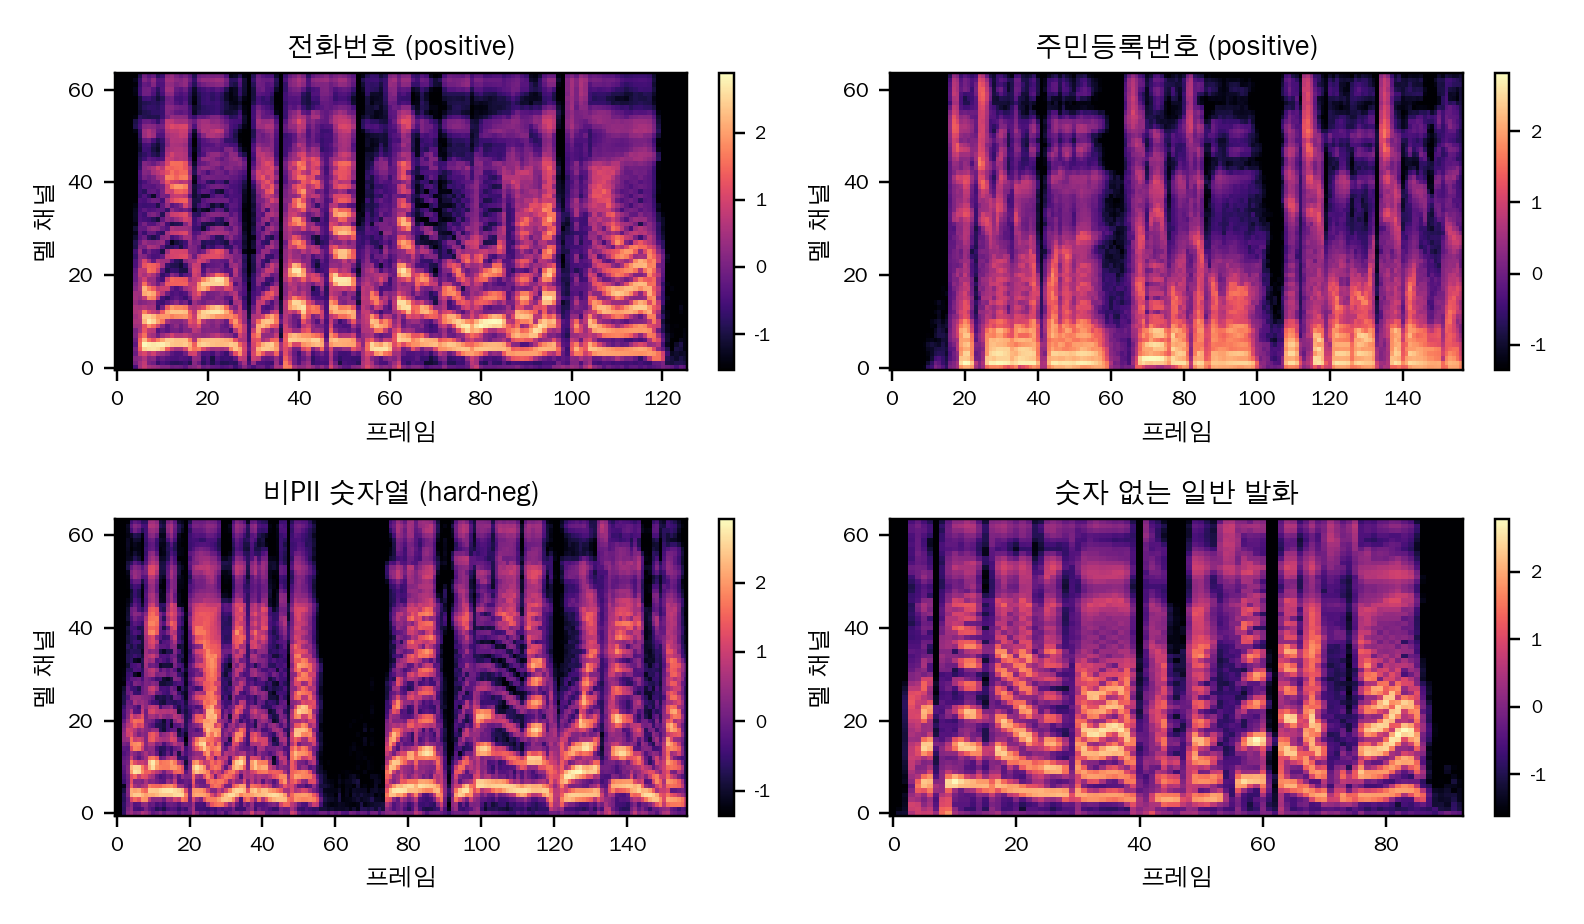
\includegraphics[width=0.88\linewidth]{melspec_examples.png}
\caption{멜 스펙트로그램 예시. v2 데이터의 네 클립(전화번호 positive, 주민등록번호
positive, hard-negative 숫자열, 숫자 없는 일반 발화)의 첫 5초 윈도를 모델 입력과 동일하게
변환한 것이다(멜 채널 64, 윈도별 표준화 후의 값). 자릿수로 낭독되는 PII 형식 숫자열은
규칙적인 시간-주파수 패턴(세로 줄무늬)으로 나타난다. 이 네 클립을 학습에서 제외한 뒤 실제로
추론했을 때 모델이 부여한 PII 확률은 각각 0.973, 0.989, 0.107, 0.030으로 네 건 모두
정답이었으므로, 그림의 텍스처 차이는 사후 해석이 아니라 모델의 판정과 일치한다.}
\label{fig:melspec}
\end{figure}

\subsection{모델과 비교군}
직접 설계한 \texttt{simple\_cnn}은 $3\times3$ 합성곱-배치정규화-ReLU-맥스풀 4블록
(채널 $16\to32\to64\to64$) 뒤에 전역 평균 풀링, 드롭아웃(0.3), 선형 분류기를 둔 60{,}706
파라미터 모델이다. 전역 평균 풀링을 사용하므로 시간축 위치에 대해 평행이동 불변에 가깝고,
숫자열이 윈도 안 어디에 놓이든 같은 특징이 활성화된다. 비교군으로는 ImageNet에서 사전학습된
MobileNetV3-Small~\cite{howard2019mobilenetv3}, EfficientNet-B0~\cite{tan2019efficientnet},
ConvNeXt-Tiny~\cite{liu2022convnext}를 사용한다. 이들은 3채널 입력을 요구하므로 1채널 멜
스펙트로그램을 3채널로 복제하여 넣고 분류기 헤드만 2클래스로 교체하였으며, 계층 동결이나
차등 학습률 없이 전 계층을 \texttt{simple\_cnn}과 동일한 설정으로 미세조정하고, 입력
정규화도 ImageNet 통계가 아닌 윈도별 표준화를 그대로 사용하였다.

\begin{table}[!htbp]
\centering
\caption{데이터 분할 구성(분할 시드 42). v2의 test(=v2-HN)에 easy-negative가 없는 것은
easy-negative 450개가 하나의 템플릿 그룹으로 묶여 학습 분할에 배정되었기 때문이다. v2는
655초짜리 반복 생성 클립 2개를 제거한 뒤의 구성이며(\ref{sec:method}장), 괄호 안은 제거
이전 구성이다. 제거로 test의 hard-negative 카테고리가 \{수 세기, 주문번호, 좌석번호\}에서
\{수 세기, 생일, 송장번호\}로 바뀐다.}
\label{tab:split}
\small
\begin{tabular}{lcccc}
\toprule
 & v1 합계 & v1 (positive/hard/easy) & v2 합계 & v2 (positive/hard/easy) \\
\midrule
train & 1{,}343 & 665 / 180 / 498 & 1{,}162 (1{,}165) & 539 / 174 / 449 \\
val   & 326     & 162 / 58 / 106  & 300 (304)         & 172 / 128 / 0   \\
test  & 331     & 173 / 62 / 96   & 336 (331) (v2-HN) & 189 / 147 / 0 \\
\bottomrule
\end{tabular}
\end{table}

\subsection{데이터 분할}\label{sec:method:split}
분할은 클립 단위가 아니라 \emph{문장 템플릿 단위}로 수행한다. 같은 템플릿에서 파생된
클립들은 숫자 값만 다르고 캐리어 문장과 어순이 동일하므로, 이들이 학습과 평가에 나뉘어
들어가면 모델이 템플릿 자체를 외워 점수가 부풀려진다. 따라서 각 \texttt{template\_id}를
하나의 그룹으로 묶어 통째로 한 분할에만 배정한다(template-disjoint). 목표 비율은
70/15/15이며, 라벨별로 목표량을 따로 채워 클래스 균형을 유지한다(label-stratified).
배정 순서는 그룹의 평균 길이 오름차순으로 하고, 매 그룹마다 현재 채움 비율
$\mathrm{cur}/\mathrm{target}$이 가장 작은 분할에 배정한다. 이렇게 하면 세 분할이 길이
스펙트럼의 전 구간을 고르게 나눠 갖게 되어(length-stratified), 길이 분포가 분할 간에
어긋나 길이 단서 통제가 무의미해지는 상황을 방지한다. test 분할은 학습, 하이퍼파라미터
선택, 조기 종료, 임계값 결정 어디에도 사용하지 않는다.

임계값 결정 규칙은 목적에 따라 셋으로 나뉜다. 첫째, \ref{sec:exp}장의 메인 성능표와 통제
평가는 튜닝 없이 고정 임계값 0.5를 사용한다. 둘째, LOSO의 튜닝 임계값은 각 폴드의 검증
분할에서 F1을 최대화하는 값을 0.05부터 0.95까지 0.05 간격의 19개 후보 중에서 고른 것이다.
셋째, 프리필터 운용표의 임계값은 검증 분할 positive 확률 분포에서 목표 재현율에 해당하는
분위수로 정한다. 세 규칙 모두 test를 참조하지 않는다. 또한 v1의 Original 평가셋(통제 이전
데이터)은 controlled 학습 분할에 포함된 파일을 제외한 뒤 사용하여, 두 manifest가 같은 원본
파일을 공유하면서 생기는 누수를 차단하였다.

표~\ref{tab:split}\는 실제 분할 결과이다. v1은 seed 42 기준 1{,}343/326/331로 나뉘었고,
test는 positive 173, hard-negative 62, easy-negative 96으로 구성된다. v2에서는 템플릿
그룹화가 평가 분할의 구성을 결정한다. easy-negative 450개는 모두 하나의 템플릿 식별자를
공유하여 한 덩어리로 학습 분할에 배정되었고, hard-negative는 템플릿 식별자가 생성 카테고리
이름이어서 카테고리 단위로 배정되었다. 그 결과 v2의 test는 positive 189개와 hard-negative
147개로만 이루어지며, hard-negative는 생일(56), 수 세기(52), 송장번호(39) 세 카테고리로
구성된다. 이하에서는 이 분할을 \textbf{v2-HN}(hard-negative 스트레스 셋)이라 부른다.
positive도 유형별 템플릿 인덱스로 묶여 전화번호 템플릿이 전부 학습·검증으로 배정되었으므로,
v2-HN의 positive는 카드 81개, 계좌 56개, 주민 52개이다.

이 구성은 세 가지 성질을 갖는다. 첫째, val과 test의 hard-negative 카테고리가 서로 겹치지
않으므로, val에서 고른 임계값은 학습·검증에서 한 번도 보지 못한 종류의 비PII 숫자열에
이식된 값이 된다(\ref{sec:exp}장에서 정량 확인). 둘째, 열 개 카테고리 중 세 개만 평가에
들어오며 \emph{어느 세 개인지가 난이도를 지배한다}. \ref{sec:method}장에서 밝힌 대로 655초
오염 클립 하나가 좌석번호 카테고리의 평균 길이를 부풀려 배정을 바꾸고 있었고, 그 클립을
제거하기 전에는 test의 hard-negative가 \{수 세기, 주문번호, 좌석번호\}였다. 카드와 충돌하도록
일부러 설계한 제품 일련번호는 어느 쪽에서도 평가에 들어오지 않는다. 셋째, 따라서 단일 분할의
hard-negative 오탐률은 모델의 속성이 아니라 분할 구성의 함수이며, 본 논문은 이를 보조 지표로만
쓰고 \ref{sec:exp:decision}절의 카테고리별 미학습 오탐률을 주 지표로 삼는다. 그 절차는 열 개
카테고리 전부를 누수 없이 평가하므로 이 편향을 받지 않는다.


\subsection{학습 설정}
최적화는 AdamW~\cite{loshchilov2019adamw}(학습률 $1\times10^{-4}$, weight decay
$1\times10^{-4}$), 손실은 클래스 가중치를 주지 않은 교차엔트로피, 배치 크기는 32, 최대 에폭은
50(v2 일반화 실험은 40)이며, 학습률은 cosine annealing~\cite{loshchilov2017sgdr}으로
감쇠시킨다. v1은 positive와 negative가 1:1로 균형 잡혀 있고, v2의 train은 positive 539 대
negative 626으로 약간 기울어져 있다(표~\ref{tab:split}). 매 에폭이 끝나면 검증 분할 전체를
클립 단위로 추론하여 고정 임계값 0.5에서 F1을 계산하고, 8에폭 동안 개선이 없으면 조기 종료한
뒤 검증 F1이 가장 높았던 시점의 가중치를 복원한다. 데이터 증강으로는 학습 시의 random-crop에
더해 보수적인 SpecAugment~\cite{park2019specaugment}를 적용하여, 주파수 마스크 1개(최대 8개
멜 채널)와 시간 마스크 1개(최대 16프레임)를 정규화 후 평균값에 해당하는 0으로 채운다.
데이터로더는 학습 시 셔플과 작업자 4개를 사용하고, 평가 시에는 클립 하나의 모든 윈도를 한
배치로 처리한다. 실험은 NVIDIA A100-SXM4-40GB 단일 GPU에서 수행하였고, 조기 종료로
\texttt{simple\_cnn}은 시드별 30--42에폭, 사전학습 백본은 10--35에폭에서 학습이 종료되었다.

표기 규약은 다음과 같다. v1의 메인 실험과 기준선은 시드 42, 43, 44로 3회 반복하므로 v1의
$\pm$는 시드 간 표준편차이다. 시드는 가중치 초기화와 증강 난수뿐 아니라 easy-negative
표본추출과 분할 시 그룹 셔플의 tie-break에도 영향을 주므로, 시드마다 평가셋 구성이 조금씩
달라진다(v1 test는 331--339개). v2의 표기 규약은 아래에서 따로 정한다.

v2 계열은 재현성을 확보하기 위해 학습 절차 자체를 결정적으로 고정하였다. 파이썬·NumPy·PyTorch
전역 시드에 더해 cuDNN 결정성 옵션(\texttt{deterministic=True}, \texttt{benchmark=False}),
결정적 알고리즘 선택(\texttt{use\_deterministic\_algorithms}), cuBLAS 작업공간, 데이터로더의
셔플 생성기와 작업자 시드를 모두 강제한다. 동일 시드로 두 차례 재학습하여 클립별 확률이 비트
단위로 일치함($\max|\Delta p| = 0$, $n=336$)을 확인하였다. 그 위에서 v2의 모든 수치는 학습 시드
42/43/44의 3회 반복으로 산출하고 평균$\pm$표준편차로 보고한다. 이때 \emph{분할 시드는 42로
고정}하고 학습 시드만 바꾸므로, v2의 $\pm$는 평가셋 구성이 아니라 순수한 학습 분산을 뜻한다.
평가셋 구성이 갖는 별개의 불확실성은 \ref{sec:exp}장의 템플릿 그룹 부트스트랩으로 따로 보고한다.

이 절차를 도입하는 과정에서 데이터 품질 문제 하나가 결과에 실제로 영향을 주고 있었음을
확인하였다. \ref{sec:data}장에서 언급한 655초짜리 TTS 반복 생성 클립 2개 가운데 하나가
hard-negative의 ``좌석번호'' 카테고리에 속해 있어 그 카테고리의 평균 길이를 극단적으로
부풀렸고, 분할 알고리즘이 그룹을 평균 길이 오름차순으로 배정하므로 이 한 클립이 평가 분할의
카테고리 구성 자체를 바꾸고 있었다. 실제로 두 클립을 제거하면 v2 test의 hard-negative
카테고리가 \{수 세기, 주문번호, 좌석번호\}에서 \{수 세기, 생일, 송장번호\}로 통째로 바뀐다.
이하의 v2 수치는 두 클립을 제거한 뒤 재생성한 분할에서 얻은 것이며, 제거 이전 분할에서의
결과도 비교를 위해 함께 보고한다. 이 사실은 \emph{단일 분할의 hard-negative 오탐률이 그
분할에 어떤 카테고리가 남았는지에 크게 의존한다}는 점을 드러내며, \ref{sec:exp}장에서
카테고리별 미학습 오탐률을 주 지표로 삼는 이유가 된다.

\subsection{기준선}
CNN이 학습을 했다고 주장하려면 최소한 다음 세 기준선을 넘어야 한다. (i) 학습 분할의 다수
클래스를 상수로 예측하는 majority. v1은 두 클래스가 1:1로 균형 잡혀 있어 다수 클래스가
동률이며 구현상 negative가 선택되므로, 재현율과 F1이 0이 된다. 이 기준선은 성능 하한이라기
보다 평가셋의 클래스 사전확률을 드러내는 참조점이며, 표~\ref{tab:main}의 PR-AUC 0.516이 곧
controlled 평가셋의 positive 비율에 해당한다. (ii) 클립 길이 하나만을 특징으로 쓰는
duration-only 로지스틱 회귀. (iii) 클립 전체에서 계산한 수작업 음향 통계 7개를 특징으로 쓰는
acoustic-LR 로지스틱 회귀이며, 특징은 클립 길이, 제곱평균제곱근(Root Mean Square, RMS) 에너지의 평균·표준편차, 영교차율의
평균·표준편차, 스펙트럼 중심의 평균·표준편차이다. 두 회귀 모두 표준화 후 L2 정규화
로지스틱 회귀에 입력한다. duration-only는 길이 단서만으로 과제가 풀리는지를, acoustic-LR는
길이에 시간 평균된 전역 음향 통계를 더해도 프레임 간 시간 구조 없이는 풀리지 않음을 각각
측정한다.

앞의 세 기준선은 모두 시간 구조를 갖지 않으므로, CNN이 이들을 능가한다는 사실은 ``시간 구조가
필요하다''까지만 말한다. 필요한 시간 구조가 실제로 얼마나 단순한지를 재기 위해 (iv) 학습
가중치가 전혀 없는 \emph{온셋 기준선}을 추가한다. 클립의 온셋 강도 곡선에서 온셋 시각을
검출하고, 인접 간격이 음절 속도 대역 안에 있으면서 서로 등간격인 연쇄를 찾아 그 길이를 점수로
쓴다. 자릿수 낭독은 등간격 단음절 연쇄이므로 이 값이 커진다. 연쇄 통계는 최장 연쇄 길이, 모든
등간격 연쇄의 온셋 총합, 전체 온셋 수의 세 가지를 두고, 대역·허용오차·임계값과 함께 검증
분할에서만 선택한다. 학습되는 파라미터는 없다. 자릿수 그룹 사이 휴지에서 연쇄가 끊기면 카드
4-4-4-4 형이 과소평가되므로 총합 변형을 함께 둔 것이며, 기준선을 불리하게 설정하지 않기 위한
조치이다.

\subsection{평가 지표와 평가셋}
지표는 F1, 재현율, 정밀도, ROC 곡선 아래 면적(Area Under the Receiver Operating
Characteristic curve, ROC-AUC), 정밀도-재현율 곡선 아래 면적(Area Under the
Precision--Recall curve, PR-AUC), hard-negative FPR, 추론 지연이다. 지연은 배치 크기 1로
$64\times157$ 무작위 입력을 워밍업 10회 뒤 50회 순전파한 평균이며, 멜 스펙트로그램 추출과
오디오 디코딩 시간은 포함하지 않는다.

평가셋은 test 분할에서 조건별로 파생한 다섯 가지를 사용한다. \texttt{controlled\_main}은
test 분할 그대로이고, \texttt{length\_matched}는 positive의 길이 히스토그램을 10개 구간으로
나눈 뒤 각 구간에서 같은 수의 negative를 표본추출하여 두 클래스의 길이 분포를 맞춘 것이며,
\texttt{hard\_negative\_only}는 easy-negative를 제거하고 positive와 hard-negative만 남긴
가장 어려운 조건이다. \texttt{stress\_5\_5}는 negative 내부의 easy:hard 비율을 1:1로 재가중한
것으로, positive:negative 균형이 깨지므로 임계값에 독립적인 지표 중심으로 해석한다.
\texttt{original}은 통제를 적용하기 이전의 데이터로, 누수 파일을 제외한 뒤 통제 설계의
필요성을 확인하는 데 사용한다.

\subsection{일반화 평가 절차}
화자 일반화는 leave-one-speaker-out(LOSO)으로 측정한다. 화자 한 명의 모든 클립을 test로
고정하고 나머지 화자의 클립을 template-disjoint로 나누어 학습과 검증에 쓰며, 검증
분할에서 임계값을 튜닝하여 고정 임계값 0.5와 비교한다. v1은 화자 3명과 시드 3회를 조합한
9회, v2는 화자 14명 각각을 시드 42/43/44로 학습하여 42회 수행하였다.

PII 유형 일반화는 held-out-PII 절차로 측정한다. 특정 유형(예: 주민등록번호)의 positive를
학습 풀에서 완전히 제거한 뒤 나머지 positive와 전체 negative로 모델을 학습하고, 제외했던
유형의 positive 225개 전부에 대해 재현율을 측정한다. 평가 대상 유형의 positive는 학습 중 한
번도 등장하지 않으므로, 이 절차가 검증하는 것은 미학습 유형에 대한 재현율이다. 반면 이
절차는 negative 전량을 학습 풀에 넣은 뒤 그 일부를 평가에 재사용하므로 negative 쪽
지표(정밀도, overall F1, ROC-AUC)는 낙관적으로 편향된다. 따라서 이들 지표는 보고하지 않으며,
negative 쪽 비용은 누수가 없는 \ref{sec:exp}장의 v2-HN hard-negative FPR을 참고값으로 삼되
학습 유형 구성이 다른 별개 조건임에 유의한다.

\subsection{STT+NLP 비교 경로의 구성}
표준 경로는 Whisper-large-v3~\cite{radford2023whisper}로 클립을 전사한 뒤(fp16, 30초 청크,
배치 16) 규칙 기반 탐지기를 적용하여 구성하였다. Whisper는 한국어 자릿수 발음을 대체로
아라비아 숫자로 정규화하지만 그룹 구분자는 발화 휴지에 따라 임의로 삽입하므로, 탐지기는
하이픈, 공백, 쉼표, 마침표를 무시하고 인접한 숫자들을 하나의 숫자열로 묶은 뒤 그 길이와
선두 패턴으로 유형을 판정한다(11자리이면서 ``01''로 시작하면 전화, 13자리면 주민등록번호,
16자리면 카드, 10--14자리면 계좌). 이를 ``형식만'' 변형이라 한다. ``형식+문맥'' 변형은
여기에 문맥 키워드를 결합하여, 형식이 일치하더라도 ``주문번호'', ``송장'', ``우편번호'',
``좌석'', ``일련번호'' 같은 비PII 키워드가 있고 PII 키워드가 없으면 negative로 되돌린다.
두 변형 모두 CNN과 \emph{동일한 test 분할}(v2-HN, $n=336$)에서 동일한 지표로 평가하였다.
디코딩 설정의 영향을 분리하기 위해 기본 설정(greedy) 외에 숫자 형식 예시를 초기 프롬프트로
주는 설정, 빔 서치(빔 5), 그리고 둘을 결합한 설정까지 네 가지에서 같은 절차를 반복하였다.

\section{실험 및 결과}\label{sec:exp}

\subsection{타당성: 기준선 초과 (RQ1)}
표~\ref{tab:main}에서 \texttt{simple\_cnn}은 $\text{F1}=0.955\pm0.010$,
$\text{ROC-AUC}=0.997\pm0.001$로 최고 성능의 기준선 acoustic-LR($0.761$ / $0.878$)을 크게
능가하였다. duration-only가 ROC-AUC 0.701에 그친 점은 길이 단서만으로는 과제가 풀리지 않음을,
acoustic-LR가 0.878에 그친 점은 길이를 포함한 전역 음향 통계로도 한계가 있음을 보인다. CNN이
이를 능가한다는 것은 전역 통계로 포착되지 않는 시간-주파수 패턴을 학습했음을 시사한다.

학습 없는 온셋 연쇄 기준선은 이 진술의 범위를 좁혀 준다. 등간격 음절 연쇄의 온셋 수를 세는
것만으로 v1에서 $\text{F1}=0.768$에 도달하여 acoustic-LR의 $0.761$을 고정 임계값 F1에서는
근소하게 앞선다(순위 성능은 ROC-AUC $0.804$ 대 $0.878$로 acoustic-LR가 앞선다). v2에서도
$\text{F1}=0.778$, ROC-AUC $0.734$이다. 즉 과제의 상당 부분은 ``자릿수처럼 규칙적으로
연쇄되는 음절을 몇 개나 세는가''라는 학습 없는 규칙으로 설명된다. 다만 CNN은 같은 조건에서
v1 $\text{F1}=0.955$/ROC-AUC $0.997$, v2 $\text{F1}=0.859$/ROC-AUC $0.938$로 순위 성능에서
$0.19$--$0.20$의 큰 폭을 남긴다. 따라서 60{,}706 파라미터의 기여는 ``시간 구조를 발견하는 것''이
아니라 ``같은 시간 구조를 훨씬 잘 정량화하는 것''으로 읽는 편이 정확하다. 이 관찰은
\ref{sec:exp:decision}절에서 모델의 결정 함수를 직접 특정하는 실험으로 이어진다.

\begin{table}[!htbp]
\centering
\caption{메인 성능 (v1 controlled 평가셋, 시드 42/43/44 평균$\pm$표준편차, 임계값 0.5).
평가셋은 v1 test 분할 전체($n=331$--$339$, 시드에 따라 다름)이며 클립 단위로 판정한다.
CNN 계열은 2.5초 간격 sliding window 확률의 최댓값을 클립 점수로 쓰고, 네 기준선은 클립
전체에서 계산한 특징을 사용한다. Hard-neg FPR은 hard-negative 클립(시드당 58--72개)만을
분모로 하는 오탐률이며, ROC-AUC와 PR-AUC는 시드 평균값이다. 온셋 연쇄 기준선만 시드 42
단일 분할에서 측정하였고, 점수가 정수값이라 PR-AUC는 보고하지 않는다. 같은 기준선의 다른
두 통계량은 최장 연쇄 길이 $\text{F1}=0.687$(ROC-AUC $0.546$), 전체 온셋 수
$\text{F1}=0.781$(ROC-AUC $0.800$)이다.}
\label{tab:main}
\footnotesize
\setlength{\tabcolsep}{4pt}
\begin{tabular}{lcccccc}
\toprule
모델 & F1 & Recall & Precision & Hard-neg FPR & ROC-AUC & PR-AUC \\
\midrule
majority (기준선)      & $0.000$ & $0.000$ & --- & $0.000$ & $0.500$ & $0.516$ \\
duration-only (기준선) & $0.633$ & $0.630$ & $0.635$ & $0.812$ & $0.701$ & $0.638$ \\
acoustic-LR (기준선)   & $0.761$ & $0.703$ & $0.832$ & $0.264$ & $0.878$ & $0.884$ \\
온셋 연쇄 (무학습 기준선) & $0.768$ & $0.821$ & $0.721$ & $0.532$ & $0.804$ & --- \\
\textbf{simple\_cnn}   & $\mathbf{0.955\pm0.010}$ & $\mathbf{0.927\pm0.028}$ & $0.986\pm0.011$ & $\mathbf{0.006\pm0.008}$ & $\mathbf{0.997}$ & $\mathbf{0.998}$ \\
mobilenet\_v3\_small   & $0.776\pm0.011$ & $0.642\pm0.012$ & $0.982\pm0.014$ & $0.021\pm0.015$ & $0.945$ & $0.954$ \\
efficientnet\_b0       & $0.867\pm0.010$ & $0.771\pm0.024$ & $0.991\pm0.013$ & $0.011\pm0.016$ & $0.994$ & $0.994$ \\
convnext\_tiny         & $0.804\pm0.132$ & $0.703\pm0.172$ & $0.959\pm0.058$ & $0.056\pm0.079$ & $0.962$ & $0.960$ \\
\bottomrule
\end{tabular}
\end{table}

\subsection{지름길 단서 통제 (RQ2)}
\textbf{길이 단서.} duration-only 기준선은 length-matched 평가셋에서 ROC-AUC가
$0.701 \to 0.534$(우연 수준)로 붕괴하고 hard-negative의 90.7\%를 positive로 오판하지만,
CNN은 같은 평가셋에서 F1이 controlled와 사실상 동일하고($0.956\pm0.011$ 대
$0.955\pm0.010$) hard-negative 오탐은 세 시드 모두 0건이었다($0.000\pm0.000$).

\textbf{숫자 존재 대 그 밖의 신호.} 날짜, 주문번호, 가격 등 비PII 숫자열에 대한 오탐률이
$0.006\pm0.008$로 매우 낮아, 판별 근거가 ``숫자가 들린다''는 사실 자체는 아님이 확인된다.
다만 이 조건만으로는 남은 신호가 무엇인지 알 수 없다. v1의 positive는 전화번호(11자리)
하나뿐이고 v1 hard-negative의 자릿수는 대부분 5 이하이므로, ``형식''과 ``자릿수 낭독의 분량''이
아직 분리되지 않은 상태이다. 이 분리는 \ref{sec:exp:decision}절에서 수행한다.
negative를 hard-negative로만 좁힌 가장 어려운 조건에서 이 대비는 오히려 더 뚜렷해진다. 이
평가셋에서 CNN의 정밀도는 $0.998\pm0.003$, ROC-AUC는 $0.9992\pm0.0006$, PR-AUC는
$0.9997\pm0.0002$로 다섯 평가셋 가운데 가장 높았던 반면, duration-only 기준선의 ROC-AUC는
$0.394$로 우연 수준 아래까지 떨어졌다. 길이 정렬을 위해 붙인 캐리어 문장 때문에
hard-negative가 오히려 positive보다 길어져 길이 단서가 역방향으로 작동하기 때문이다.
easy:hard 비율을 1:1로 올린 stress 조건에서도 CNN의 F1은 $0.958\pm0.012$, ROC-AUC $0.998$로
변하지 않았다. 즉 평가 조건을 어렵게 만들수록 지름길 기준선은 무너지고 CNN은 유지된다.

\textbf{캐리어 문장.} 길이를 맞추기 위해 hard-negative에만 붙인 캐리어 문장이 어휘·운율
상관을 새로 만들 수 있으므로, 캐리어 유무로 나눈 조건부 오탐률을 직접 검정하였다
(\ref{sec:data:pipeline}절, 표~\ref{tab:carrier}). ``캐리어가 들리면 negative''라는 지름길이
작동한다면 캐리어가 붙은 hard-negative의 오탐률이 더 낮아야 하지만, 실측은 $0.372\pm0.047$
대 $0.000$으로 정반대이며 평가 분할의 세 카테고리 안에서도 모두 같은 방향이다. 이 지름길은
부호가 반대로 기각된다.

이 confound를 설계 단계에서 없애는 방법도 검증하였다. 캐리어를 positive에도 hard-negative와
같은 확률(85\%)로 부여해 positive 900개를 전부 재합성한 데이터셋(v3)을 만들어 동일 절차로
학습하였다. 캐리어 결합률은 positive $87.0\%$, hard-negative $87.1\%$로 사실상 같아져 캐리어와
클래스의 상관은 사라진다. v3에서 성능은 $\text{F1}=0.999\pm0.001$, 재현율 $1.000$,
hard-negative 오탐률 $0.002\pm0.003$, ROC-AUC $1.000$으로 v2의 $0.859$/$0.329$와 비교가 되지
않는다.

이 차이를 어느 한 요인에 귀속할 수는 없다. v2와 v3는 세 가지가 \emph{동시에} 다르기 때문이다.
(i) 학습 시점에 캐리어가 클래스와 상관되는지 여부, (ii) 클래스 간 길이 정렬 — v3에서는 positive
길이 중앙값이 $4.56$초에서 $6.16$초로 올라 hard-negative의 $4.64$초와 벌어진다, (iii) 템플릿
그룹 분할이 낳는 평가 분할 구성 — v3의 test는 positive $172$개(v2는 $189$개)이다. 특히 (ii)는
길이를 클래스 단서로 되살리므로, v3의 높은 수치를 개선폭으로 읽어서는 안 된다.

v3 안에서 길이를 맞춘 하위집단 대비로 (ii)를 분리하려 했으나 실패하였음을 밝혀 둔다. 길이가
같은 두 집단(캐리어 없는 positive $19$개와 캐리어 있는 hard-negative $130$개, 둘 다 길이
중앙값 $4.64$초)은 총 자릿수가 각각 12--13과 0--8로 전혀 달라, 이들이 갈리는 것은
\ref{sec:exp:decision}절이 특정한 자릿수 축으로 이미 설명된다. 길이 효과를 분리하려면 자릿수를
맞춘 채 길이만 바꾼 자극이 필요하며, 그것은 \ref{sec:exp:decision}절의 통제 자극이 하는 일이다.

따라서 본 논문은 보수적인 쪽인 v2를 주 보고 대상으로 삼고, v3는 ``캐리어 얽힘을 제거하되 길이
정렬을 포기했을 때''의 참조점으로만 인용한다. 두 confound를 동시에 없애려면 캐리어를 모든
클래스에 부여하면서 캐리어 길이를 조절해 클래스 간 길이 분포까지 맞추어야 하며, 이는 향후
데이터 설계의 과제로 남는다.

\begin{table}[!htbp]
\centering
\caption{캐리어 문장 유무별 조건부 오탐률 (v2 평가 분할, \texttt{simple\_cnn}, 시드 42/43/44
평균$\pm$표준편차, 임계값 0.5). ``캐리어가 들리면 negative''라는 지름길이 작동한다면 캐리어가
붙은 쪽의 오탐률이 더 낮아야 하지만 실측은 반대이다.}
\label{tab:carrier}
\small
\begin{tabular}{lccc}
\toprule
집단 & $n$ & 오탐률(점수 $\ge 0.5$) & 평균 점수 \\
\midrule
hard-negative, 캐리어 있음 & 130 & $0.372\pm0.047$ & $0.400$ \\
hard-negative, 캐리어 없음 & 17  & $\mathbf{0.000\pm0.000}$ & $0.149$ \\
positive (캐리어 없음)      & 189 & $0.945\pm0.024$\,(=재현율) & $0.860$ \\
\bottomrule
\end{tabular}
\end{table}

이 통제가 형식적 절차가 아니었음은 통제 이전 데이터(\texttt{original} 평가셋)와 비교하면
분명해진다. 통제를 적용하지 않은 데이터에서는 클립 길이 하나만 쓰는 duration-only 기준선이
$\text{F1}=0.956$, $\text{ROC-AUC}=0.989$로 사실상 과제를 완전히 풀어 버리며, 같은 데이터에서
60{,}706 파라미터 CNN이 얻은 ROC-AUC $0.968$보다도 높다. 반면 길이 외의 전역 음향 통계에
의존하는 acoustic-LR는 통제 전 $0.876$과 통제 후 $0.878$이 사실상 같아, 통제로 제거된 것이
정확히 길이 축임을 보여준다. 낭독 방식 통제와 hard-negative 투입이 없었다면 본 연구가 보고하는
높은 성능은 전부 길이 단서로 설명될 수 있었다. 통제 이후의 수치만이 길이를 넘어선 신호를
말해 주며, 그 신호가 구체적으로 무엇인지는 \ref{sec:exp:decision}절에서 특정한다.

\subsection{결정 함수의 특정 (RQ2)}\label{sec:exp:decision}
앞 절이 배제한 것의 범위를 먼저 정확히 해 둘 필요가 있다. length-matched 평가가 보이는 것은
클립 길이가 \emph{두 클래스를 가르는} 단서로 쓰이지 않는다는 것이지, 모델이 길이에 둔감하다는
것이 아니다. 실제로는 정반대이다. hard-negative 내부에서 길이와 점수의 상관은 $0.482$로,
클래스가 같은 클립들 사이에서도 긴 클립이 더 높은 점수를 받는다. 즉 배제된 것은
``길이로 클래스를 맞힌다''는
지름길이지 ``길이가 점수에 영향을 준다''는 사실이 아니다. 숫자 존재 여부도 마찬가지로,
hard-negative가 전부 숫자를 포함하므로 그 자체로는 클래스를 가르지 못한다는 뜻이다.

그러면 두 클래스를 실제로 가르는 신호는 무엇인가. 후보는 둘이다. 하나는 논문이 겨냥한 ``PII의
형식'', 즉 자릿수 그룹 구조이고, 다른 하나는 ``자릿수 낭독이 얼마나 이어지는가''라는 분량이다.
이 절은 어느 쪽인지를 반박이 아니라 \emph{직접 측정}으로 가른다. 형식 판별기라면 같은 자릿수라도
그룹 구조가 PII 형식과 다르면 걸러야 하고, 분량 검출기라면 그룹 구조와 무관하게 자릿수 낭독의
양에만 반응해야 한다.

\paragraph{평가셋 자체가 주는 상한.}
v2-HN에서 각 클립의 자릿수 구조를 생성 규칙으로부터 복원하여 비교하면, ``자릿수 낭독으로
발음된 총 자릿수'' 하나만으로 라벨을 완벽히 분리할 수 있다(ROC-AUC $1.000$). positive는
전화 11, 계좌 12, 주민 13, 카드 16자리이고 이 분할에 남은 hard-negative는 최대 8자리이기
때문이다. 같은 평가셋에서 CNN의 ROC-AUC는 $0.938\pm0.006$이다. 즉 CNN은 자릿수 개수 임계
규칙을 \emph{근사}하고 있으며 그 규칙보다 못하다. 이 조건에서는 CNN이 형식을 추가로 쓰고
있다는 증거를 얻을 수 없다.

\paragraph{카테고리별 미학습 오탐률.}
결정 함수를 가르려면 자릿수 분량과 그룹 구조가 어긋나는 자극이 필요하다. hard-negative
카테고리를 하나씩 학습에서 완전히 제외하고 그 카테고리에 대한 오탐률을 재는 절차
(held-out-category)를 열 개 카테고리 전부에 적용하였다(표~\ref{tab:heldcat},
그림~\ref{fig:heldcat}). 이 절차는 평가 대상 카테고리가 학습에 한 번도 등장하지 않으므로
누수가 없고, 템플릿 그룹 분할이 세 개만 남기는 문제도 우회한다.

결과는 그룹 구조 가설을 분명하게 기각한다. 가장 결정적인 대비는 제품 일련번호와 주문번호이다.
제품 일련번호는 12자리를 4-4-4로 끊어 읽어 최장 연속 런이 4에 불과하지만 오탐률이
$0.947\pm0.041$로 열 카테고리 중 최고이다. 반대로 주문번호는 10자리를 끊지 않고 연속으로
읽어 최장 런이 10인데도 오탐률은 $0.622\pm0.096$에 그친다. 최장 런이 결정 변수라면 순서가
반대여야 한다. 실제로 최장 런과 오탐률의 스피어만 상관은 $0.496$에 그친다. 카드번호(16자리
4-4-4-4)의 재현율이 세 시드 모두 $1.000$인 것도 같은 그림에 맞는다. 모델은 자릿수 그룹
경계를 사실상 쓰지 않는다.

반대로 오탐률은 자릿수 낭독의 \emph{분량}에 단조 증가한다. 총 자릿수와의 상관은
$\rho=0.916$(아라비아 숫자가 없는 ``수 세기'' 제외)이다. 다만 이 축을 더 좁게 특정하는 데는
한계가 있다. 자릿수를 $N$개 읽으면 클립도 그만큼 길어지므로 총 자릿수와 클립 길이가 카테고리
수준에서 $\rho=0.869$로 공선적이고, 클립 길이와 오탐률의 상관도 $\rho=0.895$로 총 자릿수와
비슷하다. 두 변수를 관측 자료만으로 분리할 수는 없다. 카테고리 표본 수는 교란이 아니다
($\rho=-0.03$).

그럼에도 ``클립이 길어서''만으로는 설명되지 않는 부분이 있다. ``수 세기''(``하나 둘 셋 넷 다섯
여섯 일곱'')는 아라비아 숫자를 하나도 포함하지 않고 길이 중앙값이 4.28초로 생일(4.24초)과 거의
같은데, 오탐률은 $0.397\pm0.036$ 대 $0.113\pm0.051$로 세 배 넘게 높다. 길이가 같아도
등간격 단음절이 연쇄되면 점수가 오른다는 뜻이다. 즉 모델이 재는 것은 숫자 어휘도 그룹 구조도
아니고, \emph{등간격으로 연쇄되는 단음절의 분량}이다. 고유어 수사도 같은 음향 패턴을 만들기
때문에 함께 걸린다.

\begin{table}[!htbp]
\centering
\caption{hard-negative 카테고리별 미학습 오탐률 (v2, \texttt{simple\_cnn}, 시드 42/43/44
평균$\pm$표준편차, 임계값 0.5). 각 행은 그 카테고리를 학습에서 완전히 제외한 뒤 해당
카테고리 전체에 대해 측정한 값이다. ``구조''는 자릿수 그룹 길이이며 총 자릿수는 그 합이다.
참고로 positive는 전화 3-4-4(11), 계좌 3-3-6(12), 주민 6-7(13), 카드 4-4-4-4(16)이다.}
\label{tab:heldcat}
\small
\setlength{\tabcolsep}{5pt}
\begin{tabular}{lcccc}
\toprule
카테고리 & $n$ & 구조 & 총 자릿수 & 미학습 오탐률 \\
\midrule
수 세기 (count)     & 52 & --- & 0 & $0.397\pm0.036$ \\
버스번호 (bus)      & 45 & 3      & 3 & $0.030\pm0.010$ \\
좌석번호 (seat)     & 44 & 2-2    & 3 & $0.061\pm0.028$ \\
생일 (birth)        & 56 & 1-2    & 3 & $0.113\pm0.051$ \\
가격 (price)        & 43 & 5      & 5 & $0.078\pm0.011$ \\
우편번호 (postal)   & 41 & 5      & 5 & $0.114\pm0.011$ \\
날짜 (date)         & 34 & 4-1-2  & 7 & $0.225\pm0.084$ \\
송장번호 (invoice)  & 39 & 4-4    & 8 & $0.453\pm0.064$ \\
주문번호 (order)    & 45 & 10     & 10 & $0.622\pm0.096$ \\
\textbf{제품 일련번호 (serial)} & 50 & \textbf{4-4-4} & \textbf{12} & $\mathbf{0.947\pm0.041}$ \\
\bottomrule
\end{tabular}
\end{table}

\paragraph{통제 자극: 자릿수 곡선.}
앞의 두 실험은 관측 자료이므로 자릿수 분량 외의 요인(어휘, 문형)이 함께 변한다. 이를 분리하기
위해 PII 의미가 전혀 없는 순수 난수 자릿수열을 \emph{같은 TTS 백엔드와 같은 14화자}로 합성한
통제 자극 1{,}280개를 만들었다. 축은 셋이다. (A) 4/6/8/10/12/14/16자리를 끊지 않고 연속으로
읽은 것 각 100개, (B) 총 자릿수를 8/12/16으로 맞추되 카드번호처럼 4자리씩 끊어 읽은 것
(4-4, 4-4-4, 4-4-4-4) 각 100개, (C) 문틀의 기여를 분리하기 위해 문장 없이 숫자만 읽은 것 각
40개. 문틀은 ``번호는 \{v\}입니다.''로 모든 자극에서 동일하다. 채점은 v2로 학습한 세 시드의
평균 확률로 한다.

결과는 세 가지다(그림~\ref{fig:digitcurve}). 첫째, \emph{점수는 자릿수에 대한 시그모이드}이다.
문장 문틀 기준 판정 비율은 4자리 $0.00$, 8자리 $0.03$, 10자리 $0.26$, 12자리 $0.65$, 14자리
$0.89$, 16자리 $0.95$로 오르고, 로지스틱 적합의 반포화점은 $11.3$자리이다. PII 유형이
11--16자리에 몰려 있다는 사실을 생각하면, 학습이 결정 경계를 정확히 PII 구간의 하단에
놓았다는 뜻이다.

둘째, \emph{그룹 구조는 결정에 관여하지 않는다}. 총 자릿수를 맞추고 그룹만 바꾸면 판정 비율이
8자리에서 $0.03$ 대 $0.05$, 12자리에서 $0.65$ 대 $0.54$, 16자리에서 $0.95$ 대 $0.97$로 사실상
같고, 반포화점도 $11.3$ 대 $11.8$자리로 거의 겹친다. 카드번호와 같은 4-4-4-4 구조가 아무런
추가 신호도 주지 않는다는 뜻이며, \ref{sec:exp:decision}절 앞부분의 카테고리 실험과 같은
결론이다.

셋째, \emph{자릿수와 클립 길이는 둘 다 기여하며 완전히 분리되지 않는다}. 문틀을 없애면 곡선이
통째로 오른쪽으로 이동해 반포화점이 $11.3$에서 $14.8$자리로 밀린다. 숫자가 아닌 문틀 단어가
자릿수 약 3.5개분의 증거로 작용하는 셈이다. 길이가 비슷하고 자릿수만 다른 쌍을 비교하면
자릿수의 독립적 기여가 보인다. 맨숫자 14자리(3.14초, $0.450$)는 문장 10자리(3.24초, $0.260$)보다
짧으면서도 더 자주 PII로 판정되고, 맨숫자 12자리(2.79초, $0.125$)도 문장 8자리(2.89초,
$0.040$)보다 높다. 그러나 두 변수를 함께 넣은 표준화 로지스틱 회귀에서 계수는 자릿수 $1.71$,
길이 $2.17$로 길이 쪽이 오히려 약간 크다. 정확한 진술은 ``모델은 자릿수 낭독의 분량과 발화
전체의 분량을 함께 재며, 그 가운데 그룹 구조만은 쓰지 않는다''이다.

\begin{figure}[!htbp]
\centering
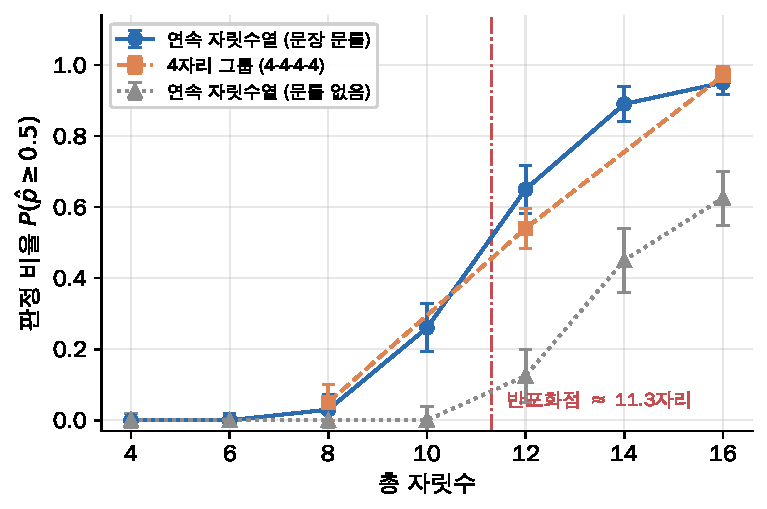
\includegraphics[width=0.66\linewidth]{digit_curve.pdf}
\caption{통제 자극에 대한 자릿수 대 판정 비율 곡선 (v2 학습 세 시드의 평균 확률, 임계값 0.5,
오차 막대는 시드 간 표준편차). 총 자릿수를 맞추고 그룹 구조만 바꾼 곡선(주황)이 연속
자릿수열(파랑)과 겹치므로 그룹 경계는 결정에 관여하지 않는다. 문틀을 제거하면(회색) 곡선이
오른쪽으로 이동해, 숫자가 아닌 문틀 단어도 점수에 기여함을 보인다.}
\label{fig:digitcurve}
\end{figure}

\begin{figure}[!htbp]
\centering
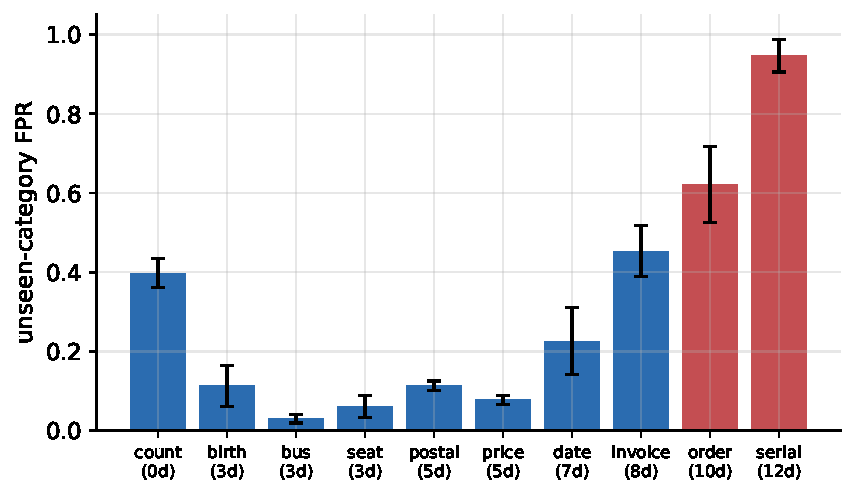
\includegraphics[width=0.72\linewidth]{heldcat_fpr.pdf}
\caption{hard-negative 카테고리별 미학습 오탐률을 총 자릿수 순으로 정렬한 것(시드 3회
평균$\pm$표준편차). 괄호 안 숫자가 총 자릿수이다. 오탐률은 총 자릿수에 단조 증가하며, 최장
연속 런이 4에 불과한 제품 일련번호(12자리)가 최장 런 10인 주문번호(10자리)보다 높다.
아라비아 숫자가 없는 수 세기는 단음절 연쇄 리듬만으로 중간 수준의 오탐을 낸다.}
\label{fig:heldcat}
\end{figure}

\subsection{모델 규모: 경량 모델의 우위 (RQ5)}
네 모델은 검증 성능에서는 구분되지 않는다. \texttt{simple\_cnn}, EfficientNet-B0,
ConvNeXt-Tiny는 세 시드 대부분에서 검증 F1 1.000에 도달했고 MobileNetV3-Small도
$0.962$--$0.991$을 기록했다. 그럼에도 test F1은 $0.776$에서 $0.955$까지 벌어지므로, 격차는
학습 데이터를 맞추는 능력이 아니라 처음 보는 템플릿으로의 일반화에서 발생한다. ConvNeXt는
두 번째 에폭에 이미 검증 F1 1.000에 도달하고 10에폭에서 조기 종료되었는데도 test F1은
$0.804\pm0.132$에 그쳤다. 임계값에 독립인 PR-AUC로 비교하면 \texttt{simple\_cnn}이 $0.998$,
ConvNeXt가 $0.960\pm0.050$, MobileNetV3가 $0.954$이다. 다만 시드 3회의 표준편차가 $0.050$에
달하므로 이 PR-AUC 차이는 통계적으로 유의하다고 주장할 수 없으며, 명확한 격차는 고정
임계값 F1과 지연에서 나타난다. 지연 측면에서는 모바일 배포를 겨냥해 설계된
MobileNetV3-Small의 $2.03$\,ms에 비해 $0.34$\,ms이고, 파라미터는 27.8M ConvNeXt-Tiny에 대해
60{,}706개이다(그림~\ref{fig:efficiency}, 표~\ref{tab:eff}).

원인으로는 네 가지를 생각할 수 있으나 근거의 강도는 서로 다르다. 실험으로 직접 관측된 것은
(1) 소량 데이터($\sim$2{,}000)에서 대형 모델의 학습이 불안정해진다는 점으로, ConvNeXt만 시드에
따라 F1이 0.635, 0.819, 0.958로 흔들려 표준편차 $\pm0.13$을 보인 반면 나머지 세 모델은
$\pm0.01$ 수준이었다. (2) ImageNet(자연 사진)과 멜 스펙트로그램의 도메인 불일치, (3) 저수준
음향 패턴으로 풀리는 과제의 단순성, (4) 작은 용량에 의한 암묵적 정규화는 해석적 가설이며,
이를 가르려면 무작위 초기화 백본과 사전학습 백본의 대조 및 용량 스윕이 필요하다.

\paragraph{학습률이 비교를 왜곡했는가.}
네 모델에 동일한 학습률 $10^{-4}$를 적용한 것이 사전학습 백본에 불리했을 가능성을 배제해야
한다. 전 계층 미세조정에 $10^{-4}$는 통상 과대하다고 알려져 있고, ConvNeXt의 큰 시드 간 분산이
바로 그 증상일 수 있기 때문이다. 이를 검정하기 위해 네 모델 각각에 $10^{-5}$, $3\times10^{-5}$,
$10^{-4}$를 시드 3회씩 적용하는 스윕을 수행하였다(총 36회, 결정성 고정, 표~\ref{tab:lrsweep}).

결과는 두 가지를 말한다. 첫째, \emph{네 모델 모두 $10^{-4}$가 최적}이며 학습률을 낮추면 오히려
성능이 떨어진다. 사전학습 백본이라고 예외가 아니다(ConvNeXt $0.776\to0.815\to0.852$,
EfficientNet $0.832\to0.824\to0.877$, MobileNetV3 $0.622\to0.776\to0.784$). 둘째, ConvNeXt의
시드 간 불안정은 학습률을 낮춰도 해소되지 않는다. 표준편차는 $10^{-4}$에서 $\pm0.116$,
$3\times10^{-5}$에서 $\pm0.072$, $10^{-5}$에서 $\pm0.067$로 줄지만 평균이 함께 떨어져 어느
설정에서도 \texttt{simple\_cnn}의 $0.952\pm0.012$에 미치지 못한다. 즉 ConvNeXt의 진동은
학습률 과대의 산물이 아니라 소량 데이터에서 대형 백본을 미세조정할 때의 성질로 보인다.

따라서 결론은 ``동일 예산·동일 설정에서''라는 단서를 ``각 모델에 가장 유리한 학습률을 고른
뒤에도''로 강화할 수 있다. 다만 이 비교군은 모두 ImageNet 사전학습 모델이며, 오디오 도메인에서
사전학습한 백본(PANNs, AST)과의 비교는 여전히 남는다. ``대규모 사전학습이 이 과제에
불리하다''가 아니라 ``ImageNet 백본은 이 과제에서 60K 전용 CNN을 넘지 못한다''가 본 실험이
지지하는 진술이다.

\begin{table}[!htbp]
\centering
\caption{학습률 스윕 (v1 controlled 평가셋, 시드 42/43/44 평균$\pm$표준편차, 임계값 0.5,
결정성 고정). 각 셀은 3회 학습의 test F1이다. 굵게 표시한 값이 모델별 최적이며 네 모델 모두
$10^{-4}$이다.}
\label{tab:lrsweep}
\small
\begin{tabular}{lccc}
\toprule
모델 & $10^{-5}$ & $3\times10^{-5}$ & $10^{-4}$ \\
\midrule
\textbf{simple\_cnn}  & $0.628\pm0.048$ & $0.756\pm0.049$ & $\mathbf{0.952\pm0.012}$ \\
mobilenet\_v3\_small  & $0.622\pm0.103$ & $0.776\pm0.003$ & $\mathbf{0.784\pm0.005}$ \\
efficientnet\_b0      & $0.832\pm0.016$ & $0.824\pm0.019$ & $\mathbf{0.877\pm0.045}$ \\
convnext\_tiny        & $0.776\pm0.067$ & $0.815\pm0.072$ & $\mathbf{0.852\pm0.116}$ \\
\bottomrule
\end{tabular}
\end{table}

\begin{figure}[!htbp]
\centering
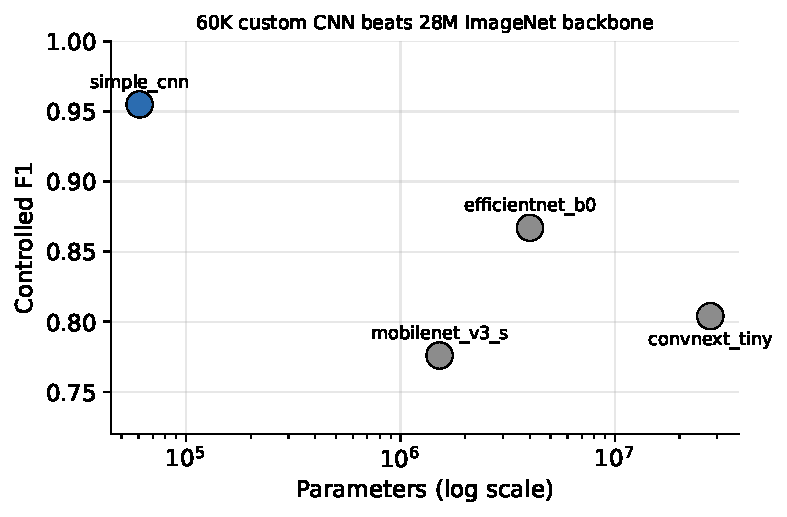
\includegraphics[width=0.58\linewidth]{efficiency.pdf}
\caption{파라미터 수(로그) 대 controlled F1(시드 3회 평균). 60K 자작 CNN이 27.8M ImageNet
백본을 능가한다.}
\label{fig:efficiency}
\end{figure}

\begin{table}[!htbp]
\centering
\caption{모델 효율성 비교. 파라미터는 학습 가능 파라미터 총수, 크기는 저장된 체크포인트 파일
용량, 지연은 NVIDIA A100 40GB에서 배치 크기 1로 $64\times157$ 입력을 워밍업 10회 뒤 50회
순전파한 평균(멜 스펙트로그램 추출 시간 제외)이다.}
\label{tab:eff}
\small
\begin{tabular}{lccc}
\toprule
모델 & 파라미터 & 크기(MB) & GPU ms/window \\
\midrule
\textbf{simple\_cnn} & \textbf{60{,}706} & \textbf{0.26} & \textbf{0.34} \\
mobilenet\_v3\_small & 1{,}519{,}906 & 6.21 & 2.03 \\
efficientnet\_b0     & 4{,}010{,}110 & 16.34 & 2.92 \\
convnext\_tiny       & 27{,}821{,}666 & 111.35 & 2.32 \\
\bottomrule
\end{tabular}
\end{table}

\subsection{화자 일반화: LOSO (RQ3)}
v1의 LOSO는 화자가 세 명뿐이라 폴드마다 두 명으로 학습하는 퇴화 조건이므로, 아래 수치는
화자 일반화의 증거라기보다 v2와의 대비를 위한 참조점으로만 읽어야 한다. 그 조건에서 미학습
화자에 대한 순위 성능은 아홉 폴드 전부에서 ROC-AUC $0.97$ 이상($0.992\pm0.008$)이었고,
negative를 hard-negative로만 좁혀도 아홉 폴드 전부 $0.98$ 이상($0.996\pm0.004$)을 유지하였다. 재현율 역시 아홉 폴드 중 여섯(Hyunsu·SunHi의 세 시드 전부)에서 정확히 1.000
이었다. 즉 판별 신호 자체는 처음 보는 화자에게도 일관되게 일반화된다.

고정 임계값 0.5에서 집계한 F1은 $0.616\pm0.280$으로 낮아 보이지만, 이는 판별 실패가 아니라
임계값 오프셋 때문이다. 평균을 끌어내린 InJoon 폴드는 세 시드 모두 재현율이
$0.068$--$0.175$로 낮은 대신 \emph{정밀도가 1.000}이었고, 임계값을 0.2에서 0.8까지 옮겨도
hard-negative 오탐이 단 한 건도 발생하지 않았다. 이 폴드의 문제는 오분류가 아니라 점수 분포
전체가 아래로 이동한 것이다. 다만 v1에서는 세 화자를 동시에 만족시키는 단일 임계값이 없다.
$\tau=0.8$에서 Hyunsu 폴드가 F1 $0.957$--$0.982$로 오르는 동안 InJoon 폴드는
$0.006$--$0.074$로 붕괴한다. 화자 수를 늘렸을 때 얻는 이득은 바로 이 지점에 있다.

화자를 3명에서 14명으로 늘리자 고정 임계값 기준 F1이 $0.871\pm0.085$로 오르고 폴드 간
표준편차가 3분의 1로 줄었다(그림~\ref{fig:loso} 좌; 14폴드 각각을 시드 42/43/44로 3회
학습한 뒤 시드 평균을 낸 값이며, $\pm$는 폴드 간 표준편차이다). 분포로 보면 성과가 더
분명하다. 14개 폴드의 F1 중앙값은 $0.893$으로 열한 폴드가 $0.87$ 이상이고, 재현율 중앙값은
$0.946$, ROC-AUC는 $0.969\pm0.021$로 열한 폴드가 $0.95$ 이상이다(그림~\ref{fig:loso} 우).
평균을 끌어내리는 것은 재현율이 $0.443$에 그친 spk13 한 폴드이며, 이 폴드조차 정밀도가
$0.934$, ROC-AUC가 $0.940$으로 순위 성능은 유지된다. 즉 실패의 성격은 판별 불능이 아니라
점수 분포의 이동이다. 운용 관점에서 더 중요한 것은 폴드별로 검증셋에서 다시 고른 임계값이
$0.35$--$0.50$(평균 $0.444\pm0.043$)의 좁은 구간에 모두 모였고, 그 임계값을 쓴 평균 F1
$0.862\pm0.083$이 고정 임계값 0.5의 $0.871\pm0.085$와 사실상 같다는 점이다. 화자가 바뀌어도
운용점을 다시 맞출 필요가 없다는 뜻이다. 다만 v1과 v2는 화자 수 외에 TTS 엔진과 PII 유형
수도 함께 달라졌으므로, 화자 수의 순효과를 분리하려면 동일 데이터에서 학습 화자 수만 바꾸는
실험이 필요하다.

\begin{figure}[!htbp]
\centering
\begin{subfigure}{0.46\linewidth}
  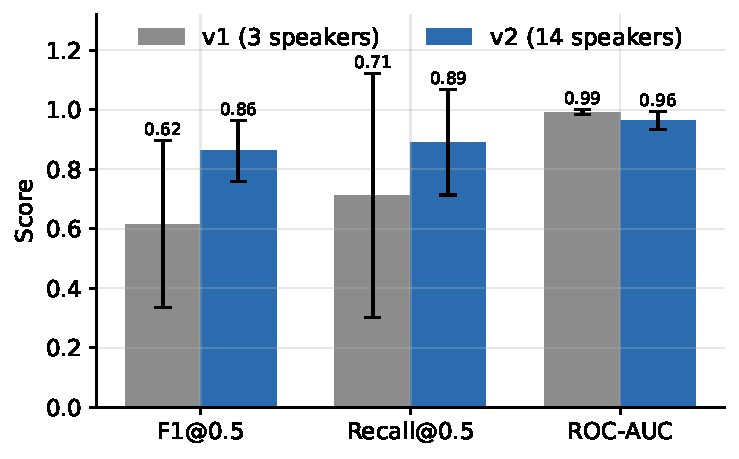
\includegraphics[width=\linewidth]{loso_v1_v2.pdf}
  \caption{v1(3화자) 대 v2(14화자)}
\end{subfigure}\hfill
\begin{subfigure}{0.52\linewidth}
  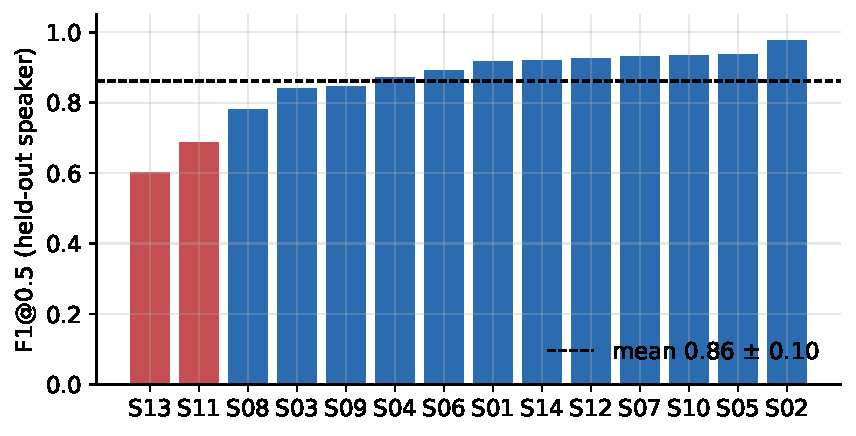
\includegraphics[width=\linewidth]{loso_folds.pdf}
  \caption{v2 화자 폴드별 F1}
\end{subfigure}
\caption{화자 분리(LOSO) 일반화(임계값 0.5, v1 9폴드·v2 14폴드). 화자 확장으로 평균 F1이
오르고 폴드 간 분산이 줄어 고정 임계값 운용이 안정화된다.}
\label{fig:loso}
\end{figure}

\subsection{PII 유형 일반화: held-out-PII (RQ3)}
각 PII 유형을 학습에서 완전히 제외하고 그 유형의 positive 225개 전부로 평가했을 때, 세 유형
모두 학습 없이 재현율 $0.89$--$0.92$를 얻었다(표~\ref{tab:heldout}). 같은 유형을 학습에
포함했을 때의 재현율이 $0.85$--$1.00$인 점을 감안하면, 유형을 통째로 빼도 재현율이 그 범위
아래로 크게 떨어지지 않는다. 학습 중 13자리 주민등록번호를 한 번도 보지 못한 모델이 그 유형의
$91.9\%$를 검출한다는 사실은, 판별 근거가 유형별 자릿수 패턴의 암기가 아님을 분명히 보여준다.

다만 이 결과가 지지하는 일반화의 \emph{내용}은 \ref{sec:exp:decision}절의 결론과 함께 읽어야
한다. 제외된 유형들은 모두 자릿수 총량이 11--16으로 학습에 남은 유형들과 같은 구간에 있다.
따라서 이 실험이 보이는 것은 ``PII 형식''이라는 추상이 유형을 넘어 전이된다는 것이 아니라,
자릿수 분량이라는 단일 축 위에서 학습된 결정 경계가 그 축의 같은 구간에 놓인 새 유형에도
그대로 적용된다는 것이다. 이는 여전히 유용한 성질이다. 새 PII 유형을 추가할 때 재학습이
필요 없다는 운용상 함의는 유지되며, 다만 그 새 유형의 자릿수 총량이 기존 구간 안에 있을
때에만 성립한다.

\begin{table}[!htbp]
\centering
\caption{held-out-PII 일반화 (v2, \texttt{simple\_cnn}, 시드 42/43/44 평균$\pm$표준편차,
임계값 0.5). 각 행은 해당 PII 유형의 positive를 학습에서 완전히 제외한 뒤 그 유형의
positive 225개 전부에 대해 측정한 재현율이다. 오른쪽 열은 같은 유형이 학습에 포함되었을 때
v2-HN에서 측정한 재현율이며, 전화번호는 v2-HN에 positive가 남지 않아 비교 대상이 없다.
``자릿수 총량''은 \ref{sec:exp:decision}절의 축에서 각 유형이 놓인 위치이다.}
\label{tab:heldout}
\small
\begin{tabular}{lcccc}
\toprule
제외한 PII & 자릿수 총량 & held-out $n$ & held-out recall@0.5 & (참고) 학습에 포함 시 recall \\
\midrule
주민번호 (rrn)     & 13 & 225 & $0.919\pm0.008$ & $0.846\pm0.042$ ($n=52$) \\
카드 (card)        & 16 & 225 & $0.902\pm0.010$ & $1.000\pm0.000$ ($n=81$) \\
계좌 (account)     & 12 & 225 & $0.893\pm0.038$ & $0.958\pm0.030$ ($n=56$) \\
\bottomrule
\end{tabular}
\end{table}

\subsection{프리필터 가치}
프리필터의 목적은 목표 재현율을 지키면서 STT 호출을 줄이는 것이다. v1 평가셋에서는 고정
임계값 0.5에서 이미 재현율 $0.927$, 정밀도 $0.986$을 유지하며 STT 호출을 51.5\% 줄일 수 있고,
임계값을 0.3으로 낮추면 재현율 $0.994$에서 44.9\%, 0.2에서는 재현율 $0.998$(세 시드 중 둘은
정확히 1.000)에서 41.6\%를 절감한다. 반대로 임계값을 0.7로 올리면 세 시드 모두 정밀도
1.000과 hard-negative 오탐 0건을 유지한 채 평균 62\%를 절감하지만, 재현율이 $0.728$로
떨어져 PII의 27\%를 놓친다. 프리필터로서 실제로 쓸 수 있는 구간은 재현율을 지키는 저임계값
쪽이며, 그 구간에서 41--45\%의 절감이 확보된다.

숫자를 포함한 발화만으로 구성된 v2-HN에서도 임계값 $0.375\pm0.059$에서 재현율
$0.981\pm0.005$를 유지하며 STT 호출을 $24.2\%$ 줄일 수 있다(표~\ref{tab:prefilter}). 주목할
점은 이 임계값들이 모두 검증 분할의 확률 분위수만으로 정해졌고 test를 참조하지 않았음에도
목표를 초과 달성했다는 것이다. 목표 재현율 $0.99$에 해당하는 임계값이 test에서
$0.996\pm0.005$를, $0.95$ 목표가 $0.981$을, $0.90$ 목표가 $0.942$를 달성하였다.
\ref{sec:method:split}절에서 밝혔듯 val과 test의 hard-negative 카테고리는 서로 겹치지 않는다.
이 성질은 의도한 설계가 아니라 템플릿 그룹화가 낳은 부작용이지만, 결과적으로 운용점이
학습·검증에서 한 번도 보지 못한 종류의 비PII 숫자열에 대해서도 이식됨을 보여준다. 다만
임계값 자체의 시드 간 변동은 작지 않으므로($0.99$ 목표에서 $0.214\pm0.047$), 프리필터
임계값은 배포 시점의 검증 데이터에서 다시 정하는 것이 안전하다.

v2-HN의 호출률은 모든 입력이 숫자를 포함하는 최악 트래픽을 가정한 값이라 운용 절감률을 크게
과소평가한다. 실제 트래픽에서의 값은 PII 발생률과 숫자 포함 비율의 함수이므로, 다음 절에서
비용 모형으로 일반화한다.

\begin{table}[!htbp]
\centering
\caption{프리필터 운용점 (v2-HN, \texttt{simple\_cnn}, 시드 42/43/44 평균$\pm$표준편차). 각
행의 임계값은 검증 분할에서 목표 재현율에 해당하는 분위수로 정한 값이다. STT 호출률은 클립
점수가 임계값 이상이어서 후단 STT로 넘어가는 클립의 비율이며 $1-\text{호출률}$이 절감률이다.
v2-HN은 숫자가 없는 easy-negative를 포함하지 않으므로, 여기의 호출률은 모든 입력이 숫자를
포함하는 최악 트래픽을 가정한 값이다. 일반 트래픽에서의 값은 표~\ref{tab:cost} 참조.}
\label{tab:prefilter}
\small
\begin{tabular}{lccccc}
\toprule
목표 재현율 & 임계값 & Recall & Precision & Hard-neg FPR & STT 호출률 \\
\midrule
0.99 & $0.214\pm0.047$ & $0.996\pm0.005$ & $0.665\pm0.014$ & $0.646\pm0.044$ & $0.843\pm0.022$ \\
0.95 & $0.375\pm0.059$ & $0.981\pm0.005$ & $0.728\pm0.015$ & $0.472\pm0.037$ & $0.758\pm0.019$ \\
0.90 & $0.500\pm0.028$ & $0.942\pm0.020$ & $0.799\pm0.006$ & $0.304\pm0.014$ & $0.663\pm0.015$ \\
\bottomrule
\end{tabular}
\end{table}


\subsection{CNN 대 STT+NLP (RQ4)}
동일 인스턴스(v2 평가 분할, $n=336$)에서 두 접근을 비교하면 강점이 뚜렷하게 갈린다
(표~\ref{tab:vs}, 그림~\ref{fig:vs}). STT+NLP는 정밀도 $1.000$과 F1 $0.964$로 앞서고, CNN은
재현율($0.945$ 대 $0.931$)과 세 자릿수 빠른 지연으로 앞선다. 이 분할의 hard-negative는 최대
8자리여서 형식 규칙을 아예 건드리지 않으므로 STT+NLP의 오탐률이 $0.000$이고, 그 결과 문맥
결합이 개입할 여지도 없다(``형식만''과 ``형식+문맥''이 동일). 형식이 충돌하는 10자리
주문번호가 평가에 포함된 제거 이전 분할에서는 ``형식만''의 오탐률이 $0.218$, 문맥 결합 시
$0.063$으로, 문맥이 형식 충돌을 해결하는 효과가 나타난다. 즉 STT+NLP의 정밀도 우위 역시
평가 분할의 자릿수 구성에 의존한다.

\paragraph{전사 취약성은 설정 미조정인가.}
논문이 STT의 약점을 ``구조적''이라고 부르려면 최소한 서로 다른 디코딩 설정에서 같은 실패가
재현되어야 한다. 기본 설정 외에 숫자 형식 예시를 초기 프롬프트로 준 설정, 빔 서치(5), 그리고
둘을 결합한 설정까지 네 가지에서 유형별 재현율을 측정하였다(표~\ref{tab:vs}). 16자리
카드번호 재현율은 네 설정에서 각각 $0.864$, $0.802$, $0.852$, $0.815$로, 프롬프트나 빔 서치가
이 실패를 개선하지 못한다. 오히려 형식 예시를 준 프롬프트 설정이 가장 낮다. 반면 13자리
주민등록번호는 네 설정 모두 $1.000$이다. 즉 실패는 디코딩 탐색의 문제가 아니라 자릿수가
길어질수록 전사가 숫자를 병합·분절·누락하는 데서 오는 것이며, ``구조적''이라는 규정이
유지된다. 같은 인스턴스에서 CNN의 카드 재현율은 세 시드 모두 $1.000$이다.

유형별로 나누면 상보성이 선명해진다. CNN이 우위를 보이는 지점은 정확히 전사가 취약한 긴
숫자열(카드 16자리: $1.000$ 대 $0.802$--$0.864$)이고, STT+NLP가 앞서는 지점은 짧고 문맥
키워드가 뚜렷한 유형(주민 13자리: $1.000$ 대 $0.846\pm0.042$)이다. 두 경로를 직렬로 결합할
근거가 여기에 있다.

이 비교에서 STT+NLP 쪽 조건도 밝혀 둔다. 합성음에서는 Whisper 전사가 거의 완벽하여(일반 발화
449개 기준 WER 중앙값 $0$, 평균 $0.079$, 완전일치 $80.8\%$) STT+NLP 성능은 best-case 상한이다.
이는 초기 실험에서 쓴 청크 기반 파이프라인 대비 개선된 값이다. 당시에는 반복 루프 형태의 환각이
1건 발생해 평균 WER이 $0.722$까지 올랐는데, 30초 청크 분할 없이 모델을 직접 호출하는 본
측정에서는 환각이 0건이었다. 즉 그 환각은 전사 자체의 한계가 아니라 장문 디코딩 절차의
산물이었다. 완전일치하지 않은 클립이 여전히 $19.2\%$라는 점은 남는다. 중앙값이 0이라는 사실은
전사 오류가 사라졌다는 뜻이 아니라 소수
구간에 집중되어 있다는 뜻이며, 그 소수 구간이 하필 긴 숫자열이라는 점이 카드번호 재현율
$0.802$--$0.864$로 나타난다. 실통화 조건에서의 상대 열화는 \ref{sec:exp:degrade}절의 열화
데이터를 두 경로에 함께 적용해 측정하였다. 8\,kHz 협대역과 G.711 왕복에서 CNN의 F1은
$0.859\to0.831$, STT+NLP는 $0.964\to0.956$으로 \emph{양쪽 모두 견딘다}. 즉 채널 요인만
놓고 보면 격차의 방향이 바뀌지 않는다. 반면 가산 잡음에서는 방향이 갈리며, 그
비교는 \ref{sec:exp:degrade}절에서 다룬다.


\begin{table}[!htbp]
\centering
\caption{CNN 대 STT+NLP, 네 가지 Whisper 디코딩 설정 (v2 평가 분할, $n=336$, 임계값 0.5).
CNN은 시드 42/43/44 평균$\pm$표준편차이다. 이 분할의 hard-negative는 최대 8자리여서 형식
규칙을 건드리지 않으므로 STT+NLP의 ``형식만''과 ``형식+문맥''이 동일한 값을 낸다. 유형별
재현율에서 16자리 카드번호만 네 설정 모두에서 무너진다는 점이 핵심이다. 지연은 NVIDIA A100
40GB 기준으로 CNN이 배치 1의 윈도당 $0.344$\,ms(전처리 제외)이다. Whisper는 본 절의 재측정에서
빔 서치(5) 클립당 $0.541$\,s, 빔+프롬프트 $0.674$\,s였으며, 기본 설정의 $0.360$\,s는 초기
청크 기반 파이프라인에서 측정한 값이라 나머지와 측정 조건이 다르다. 세 자릿수라는 지연 격차의
크기는 어느 값을 쓰든 바뀌지 않는다.}
\label{tab:vs}
\footnotesize
\setlength{\tabcolsep}{4pt}
\begin{tabular}{lcccccc}
\toprule
접근 & F1 & Recall & Precision & 주민(13) & 계좌(12) & 카드(16) \\
\midrule
CNN (음향) & $0.859\pm0.011$ & $\mathbf{0.945\pm0.019}$ & $0.787\pm0.016$ & $0.846$ & $0.958$ & $\mathbf{1.000}$ \\
\midrule
STT+NLP, 기본            & $\mathbf{0.964}$ & $0.931$ & $\mathbf{1.000}$ & $1.000$ & $0.964$ & $0.864$ \\
STT+NLP, 프롬프트        & $0.956$ & $0.915$ & $\mathbf{1.000}$ & $1.000$ & $1.000$ & $0.802$ \\
STT+NLP, 빔 서치(5)      & $0.959$ & $0.921$ & $\mathbf{1.000}$ & $1.000$ & $0.946$ & $0.852$ \\
STT+NLP, 빔+프롬프트     & $0.959$ & $0.921$ & $\mathbf{1.000}$ & $1.000$ & $1.000$ & $0.815$ \\
\bottomrule
\end{tabular}
\end{table}

\begin{figure}[!htbp]
\centering
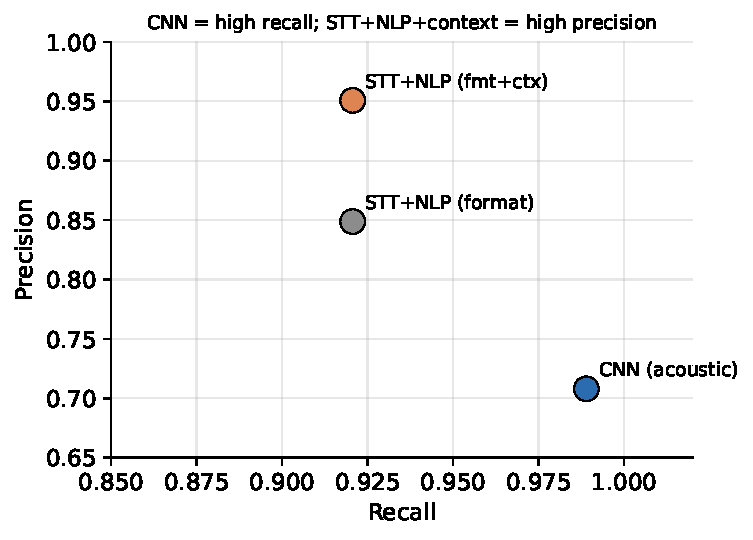
\includegraphics[width=0.58\linewidth]{cnn_vs_sttnlp.pdf}
\caption{재현율-정밀도 트레이드오프(v2-HN, $n=336$). CNN은 고재현율, STT+NLP는 고정밀도로
상보적이며, 네 디코딩 설정이 모두 같은 영역에 모인다.}
\label{fig:vs}
\end{figure}

\subsection{협대역·코덱·잡음 열화}\label{sec:exp:degrade}
실험은 16\,kHz 광대역 합성음에서 수행되었지만 표적 도메인은 8\,kHz 협대역 전화망이다. 새
데이터 수집 없이 이 격차의 크기를 재기 위해, v2 평가 분할의 클립을 전화망 조건으로 열화시킨
뒤 동일 체크포인트로 재평가하였다(표~\ref{tab:degrade}). 조건은 8\,kHz 리샘플 왕복(nb8k),
여기에 G.711 $\mu$-law 부호화를 더한 것(g711), 그리고 각 조건에 백색잡음을 SNR 20/10\,dB로
더한 것이다.

결과는 두 요인의 기여를 뚜렷하게 분리한다. \emph{대역 제한과 코덱은 거의 무해하다.} 8\,kHz
리샘플만으로는 F1이 $0.859\to0.849$, ROC-AUC가 $0.938\to0.920$으로 거의 변하지 않고, G.711
양자화를 더해도 $0.831$ / $0.914$에 머문다. 자릿수 낭독의 판별 정보가 4\,kHz 이하의 저역
포먼트와 음절 리듬에 실려 있음을 생각하면 자연스러운 결과이다.

\paragraph{잡음을 어느 대역에 넣는가가 결론을 바꾼다.}
가산 잡음 조건에서는 잡음의 대역이 결정적이다. 협대역 채널을 통과한 신호는 4\,kHz 이상 에너지가
사실상 0이므로(본 데이터의 G.711 클립 336개에서 4\,kHz 이상 에너지 비율의 중앙값 $1.3\times10^{-5}$,
최댓값 $1.3\times10^{-4}$), 전대역 백색잡음을 공칭 SNR로
주입하면 잡음 전력의 절반이 \emph{신호가 전혀 없는 대역}에 떨어진다. 그 대역은 64채널 멜
필터뱅크의 절반을 차지하므로 모델 입력에는 크게 반영된다. 실제 전화망은 이런 잡음을 전달하지
못한다. 따라서 잡음은 전화 통과대역(300--3400\,Hz)으로 제한하고 SNR도 대역 내 전력비로
정의하는 것이 옳으며, 본 절은 두 방식을 모두 보고한다(표~\ref{tab:degrade}).

이 구분이 결론을 뒤집는다. 전대역 잡음에서는 공칭 SNR 20\,dB만으로 재현율이
$0.945\to0.418$로 무너지지만, 통과대역 잡음 20\,dB에서는 $0.931\pm0.069$로 거의 유지된다.
두 SNR은 정의가 달라 직접 비교할 수 없다는 점을 밝혀 둔다. 통과대역 SNR은 대역 내 전력비이고
G.711 클립에서 300--3400\,Hz가 총전력의 약 $52\%$이므로, 통과대역 20\,dB는 전체 전력 기준으로는
약 $24$\,dB에 해당한다. 이 $4$\,dB 차이만으로는 $0.418$과 $0.931$의 간극이 설명되지 않으므로
지배적 요인은 잡음의 대역 배치이다. 전대역 조건에서 SNR을 10\,dB로 더 낮추면 재현율이 오히려
$0.589$로 오르는데, 이 비단조성 역시 손실이 정보량이 아니라 점수 분포 이동에서 온다는 해석과
맞는다. 즉 ``가산
잡음이 음향 프리필터를 무너뜨린다''는 서술은 표적 도메인이 물리적으로 만들 수 없는 대역 외
잡음에 기댄 것이었다. 통과대역 조건에서 실제로 무너지는 것은 재현율이 아니라 \emph{정밀도와
운용점의 안정성}이다. hard-negative 오탐률이 $0.329\to0.689$로 오르고, SNR을 10\,dB와
5\,dB로 낮추면 시드 간 재현율이 각각 $[0.989, 1.000, 0.249]$, $[1.000, 1.000, 0.000]$로
극단적으로 갈린다. 판별 능력도 ROC-AUC $0.938\to0.804/0.770/0.742$로 유의하게 떨어지지만(우연 대비 여유가
$0.438\to0.242$로 $45\%$ 감소), 시드 간 재현율이 $1.000$과 $0.000$으로 갈리는 폭은 그 감소만으로
설명되지 않는다. 지배적 요인은 점수 분포가 잡음 수준에 따라 예측 불가능하게 이동하여 고정
임계값이 무의미해지는 데 있다.
프리필터 관점에서 재현율 손실과 정밀도 손실은 비용이 전혀 다르다. 전자는 PII 누락이고 후자는
STT 호출 증가일 뿐이므로, 통과대역 조건의 열화는 앞의 서술이 시사하던 것보다 훨씬 덜 치명적이다.

\paragraph{잡음 증강 학습으로 회복되는가.}
위 열화는 모두 평가 시점에만 가해졌고 모델은 깨끗한 16\,kHz 합성음만 보았다. 관측된 저하가
과제의 한계인지 학습 조건 불일치인지 가르기 위해, 학습 데이터의 절반에 확률적으로 대역 제한,
$\mu$-law 양자화, 통과대역 잡음(SNR 5--25\,dB)을 섞어 동일 절차로 재학습하였다(시드 3회).

다만 이 실험이 무엇을 보이는지는 정확히 한정해야 한다. 증강에 쓴 통과대역 잡음은 평가에 쓴
것과 대역 상수·필터·잡음원·SNR 정의가 같고 학습 SNR 범위 $[5, 25]$\,dB가 평가점 $\{20, 10, 5\}$을
모두 포함한다. 따라서 아래 회복치는 \emph{정합 조건에서의 상한}이며, 처음 보는 잡음 종류로의
일반화를 뜻하지 않는다. 실제로 학습에 넣지 않은 전대역 잡음에서는 증강이 오히려 성능을 낮춘다
(표~\ref{tab:degrade} 맨 아래 두 행: F1 $0.542\to0.435$).

그 한정 아래에서 효과는 분명하다(표~\ref{tab:degrade} 가운데 열). 통과대역 잡음 조건에서
F1은 SNR 20, 10, 5\,dB에 대해 각각 $0.757$, $0.770$, $0.777$로 \emph{SNR에 거의 무관하게}
평평해지고, 재현율도 $0.843$, $0.838$, $0.785$로 안정된다. 기본 모델의 $0.754$, $0.622$,
$0.491$과 비교하면 SNR 5\,dB에서 F1이 $0.29$ 오른다. 시드 간 표준편차도 $\pm0.348$에서 $\pm0.024$로 줄어 운용점 불안정이
해소된다. 대가는 깨끗한 조건의 성능으로, F1이 $0.859\to0.807$, 재현율이 $0.945\to0.885$로
내려가고, ROC-AUC도 $0.938\to0.883$으로 함께 내려간다. 또 SNR 20\,dB에서는 증강의 이득이
사실상 없다(F1 $0.754\to0.757$, 재현율은 $0.931\to0.843$으로 오히려 내려간다). 즉 증강은
\emph{낮은 SNR에서의 붕괴와 시드 간 불안정}을 없애는 대신 깨끗한 구간의 성능을 내주는 거래이며, 잡음 하 붕괴가 최소한 정합 조건에서는 과제의
본질이 아니라 학습 조건 불일치였음을 보인다.

\paragraph{같은 열화에서 STT+NLP.}
동일 클립에 STT+NLP 경로를 적용하면 이 경로가 전 조건에서 훨씬 견고하다. 통과대역 잡음
20/10/5\,dB에서 F1이 $0.962$/$0.950$/$0.932$로, 5\,dB에서만 소폭 내려간다. 16자리 카드
재현율도 $0.840$/$0.790$/$0.728$로 유지된다. 대규모 실음성으로 학습된 ASR과 깨끗한 합성음
1{,}800개로 학습된 60{,}706 파라미터 CNN을 견주는 비대칭 비교이므로 이 격차를 두 \emph{접근}의
차이로 읽어서는 안 되지만, 운용 판단에는 그대로 반영되어야 한다. 잡음이 있는 구간에서 음향
프리필터가 STT+NLP보다 잃을 것이 많다는 사실은 변하지 않는다.

\begin{figure}[!htbp]
\centering
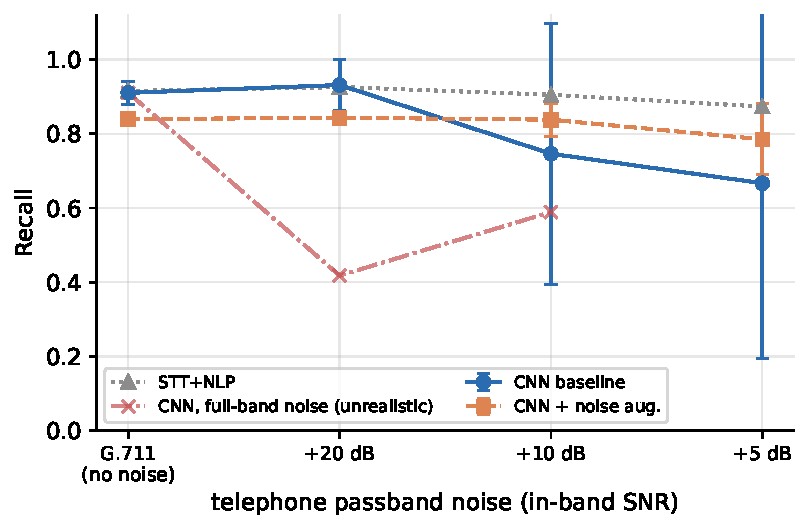
\includegraphics[width=0.68\linewidth]{degradation.pdf}
\caption{열화 조건별 재현율. 잡음을 전화 통과대역으로 제한한 조건(실선)에서는 기본 모델의
재현율이 SNR 20\,dB까지 유지되지만 그 아래에서 시드에 따라 극단적으로 갈리고, 잡음 증강 학습
모델(파선)은 SNR 전 구간에서 평평하다. 회색은 신호가 없는 대역까지 잡음을 넣은 전대역 조건으로,
표적 도메인에서는 발생하지 않는다.}
\label{fig:degradation}
\end{figure}

이 결과는 \ref{sec:discuss}장의 2단계 파이프라인 제안에 조건을 붙이되, 초기 측정이 시사하던
것보다 완만한 조건을 붙인다. 전화망이 실제로 전달하는 통과대역 잡음에서 기본 모델의 재현율은
SNR 20\,dB까지 $0.931$로 유지되고, 증강 학습을 적용하면 SNR 5\,dB까지 F1이 $0.777$로
평평해진다. 따라서 프리필터의 운용 전제는 ``잡음이 없어야 한다''가 아니라 ``잡음 조건으로 증강
학습하고, 깨끗한 구간의 F1 $0.05$를 대가로 지불한다''이다. 다만 같은 조건에서 STT+NLP가
$0.932$--$0.962$를 유지하므로, 잡음 구간에서 프리필터가 더 많이 잃는다는 사실 자체는 변하지
않는다. 또한 여기서 쓴 잡음은 정상 백색잡음이므로, 실제 통화의 배경 대화·음악 같은 비정상
잡음에서 같은 결과가 나온다고 단정할 수는 없다.

\begin{table}[!htbp]
\centering
\caption{협대역·코덱·잡음 열화 후 성능 (v2 평가 분할 $n=336$, 임계값 0.5, 시드 42/43/44
평균$\pm$표준편차). 열화는 평가 시점에만 가하며, ``기본''은 깨끗한 음성만으로 학습한 모델,
``증강''은 학습 데이터의 절반에 대역 제한·$\mu$-law·통과대역 잡음을 섞어 학습한 모델이다.
STT+NLP는 기본 디코딩 설정의 ``형식+문맥'' 변형이며 단일 실행이다. 통과대역 잡음은
300--3400\,Hz로 제한하고 SNR을 대역 내 전력비로 정의한 것으로, 전화망이 실제로 전달하는
조건이다. 맨 아래 두 행의 전대역 잡음은 신호가 없는 4--8\,kHz에 잡음의 절반이 떨어지므로
표적 도메인에서는 발생하지 않는다.}
\label{tab:degrade}
\footnotesize
\setlength{\tabcolsep}{4pt}
\begin{tabular}{lcc|cc|c}
\toprule
 & \multicolumn{2}{c|}{CNN 기본} & \multicolumn{2}{c|}{CNN 잡음 증강} & STT+NLP \\
조건 & F1 & Recall & F1 & Recall & F1 \\
\midrule
clean (16\,kHz) & $0.859\pm0.011$ & $0.945\pm0.019$ & $0.807\pm0.010$ & $0.885\pm0.026$ & $0.964$ \\
8\,kHz 왕복 & $0.849\pm0.016$ & $0.910\pm0.030$ & $0.819\pm0.015$ & $0.834\pm0.025$ & $0.947$ \\
G.711 ($\mu$-law) & $0.831\pm0.013$ & $0.910\pm0.031$ & $0.806\pm0.015$ & $0.840\pm0.002$ & $0.956$ \\
\midrule
\;+ 통과대역 잡음 20\,dB & $0.754\pm0.020$ & $0.931\pm0.069$ & $0.757\pm0.002$ & $0.843\pm0.002$ & $0.962$ \\
\;+ 통과대역 잡음 10\,dB & $0.622\pm0.169$ & $0.746\pm0.352$ & $\mathbf{0.770\pm0.010}$ & $0.838\pm0.044$ & $0.950$ \\
\;+ 통과대역 잡음 5\,dB & $0.491\pm0.348$ & $0.667\pm0.471$ & $\mathbf{0.777\pm0.024}$ & $0.785\pm0.096$ & $0.932$ \\
\midrule
\;+ (참고) 전대역 잡음 20\,dB & $0.542\pm0.116$ & $0.418\pm0.127$ & $0.435\pm0.231$ & $0.381\pm0.303$ & $0.967$ \\
\;+ (참고) 전대역 잡음 10\,dB & $0.615\pm0.111$ & $0.589\pm0.180$ & $0.620\pm0.100$ & $0.653\pm0.227$ & $0.953$ \\
\bottomrule
\end{tabular}
\end{table}

\section{논의}\label{sec:discuss}

\subsection{정밀도 약점의 원인 진단}
\ref{sec:exp:decision}절의 결론을 정밀도 문제로 옮기면 진단이 단순해진다. 모델이 재는 것이
자릿수 낭독의 분량이라면, PII와 그 분량이 겹치는 비PII 숫자열은 이 결정 축 위에서 구분할 수
없다. 실제로 제품 일련번호(12자리)는 계좌번호(12자리)와 총량이 정확히 같고 미학습 오탐률이
$0.947$이다. 다만 두 유형은 그룹 구조가 4-4-4 대 3-3-6으로 다르므로, 이것은 \emph{과제}가
아니라 \emph{현재 모델이 학습한 표현}의 한계이다. 즉 정밀도 개선의 여지는 남아 있으며, 그
방향은 그룹 경계를 결정에 실제로 반영하도록 만드는 것이다. 문맥을 보는 후단이 필요한 이유는
그와 별개로, 형식이 같아도 문맥상 PII가 아닌 경우가 존재하기 때문이다.

이 관점은 단일 분할에서 측정한 hard-negative 오탐률을 어떻게 읽어야 하는지도 결정한다. 그
값은 모델의 속성이라기보다 \emph{평가 분할에 어떤 카테고리가 남았는지}의 함수이다. 같은
학습 절차로 같은 데이터를 쓰되 분할만 달리한 두 계열을 비교하면, 655초 오염 클립을 제거한
분할에서는 $0.329\pm0.034$, 제거 이전 분할에서는 $0.566\pm0.041$로 0.24가 벌어진다. 전자의
평가 카테고리는 \{생일 $0.167$, 수 세기 $0.404$, 송장번호 $0.462$\}이고 후자는 \{좌석번호
$0.222$, 수 세기 $0.577$, 주문번호 $0.896$\}이다. 템플릿 그룹 단위 부트스트랩으로 재면 이
불확실성이 정량화된다. 오탐률의 95\% 구간은 $[0.167, 0.466]$, 정밀도는 $[0.363, 0.967]$로,
시드 간 표준편차($\pm0.034$, $\pm0.016$)보다 한 자릿수 크다. 다만 이 평가 분할의 템플릿
그룹은 여섯 개(positive 세 유형, hard-negative 세 카테고리)뿐이므로 재표집 단위가 적고,
따라서 이 구간은 정확한 피복률을 갖는 신뢰구간이라기보다 \emph{불확실성의 하한}으로 읽어야
한다. 그럼에도 시드 분산과의 자릿수 차이는 이 정도 표본으로도 분명하다. 즉 v2의 지배적 불확실성 축은
학습 난수가 아니라 평가에 어떤 템플릿이 들어오는가이며, 단일 분할의 오탐률 하나를 모델의
정밀도로 인용해서는 안 된다. 표~\ref{tab:heldcat}의 카테고리별 미학습 오탐률이 이 지표를
대체해야 한다.

v1에서 같은 지표가 $0.006$이었던 것도 같은 틀로 설명된다. v1의 positive는 전화번호(11자리)
하나뿐이고 v1 hard-negative 카테고리의 자릿수 총량은 대부분 5 이하여서, 자릿수 총량 축에서
두 클래스가 거의 겹치지 않는다. v2에서 계좌(12)와 카드(16)를 추가하자 12자리 제품 일련번호와
10자리 주문번호가 곧바로 충돌 구간으로 들어왔다. 두 수치의 비를 악화 배수로 읽는 것은
과대해석이며, ``PII 유형을 늘리면 자릿수 총량이 겹치는 negative가 늘어난다''가 정확한 진술이다.

보정의 성격도 함께 확인된다. 보정 파라미터는 검증 분할에서 적합하고 test에서 평가하였다.
기대 보정 오차(Expected Calibration Error, ECE)는 $0.098\pm0.012$로 절대적으로 낮지 않지만,
온도 스케일링($T=0.67\pm0.07$)을 적용해도 $0.097\pm0.014$로 변화가 없고 Platt
스케일링~\cite{guo2017calibration}은 $0.110\pm0.010$으로 오히려 악화된다. 온도 스케일링은
순위를 보존하는 단조 변환이므로 임계값 0.5에서의 재현율·정밀도·호출률도 보정 전후로 동일하다.
운용상으로는 사후 보정 단계를 추가할 실익이 없다는 뜻이고, 진단상으로는 정밀도 개선의 레버가
보정이 아니라 (a) 문맥 단서 결합, (b) 자릿수 총량이 겹치는 충돌형 hard-negative의 강화
학습에 있음을 뜻한다.

\subsection{설계 함의: 2단계 파이프라인}
실험 결과 CNN은 고재현율·초저비용, STT+NLP(형식+문맥)는 고정밀·문맥 강함으로 상보적이며,
표~\ref{tab:vs}\가 보이듯 두 접근이 실패하는 유형까지 서로 어긋난다. 따라서 CNN으로 1차
선별(고재현율로 후보를 거르고 명백한 비PII는 조기 종료)한 뒤 남은 후보에만 STT+NLP를 적용해
정밀 확정하는 2단계 파이프라인이 두 접근의 장점을 결합한다. 절감되는 STT 비용은 트래픽
구성에 따라 달라지며, 모든 발화가 숫자를 포함하는 최악 조건에서 약 24\%, easy-negative가
섞인 v1 조건에서 41.6--51.5\%로 측정되었다. 일반 트래픽에서의 값은
\ref{sec:discuss:cost}절의 비용 모형으로 추정한다.

다만 이 제안에는 명시적인 전제가 붙는다. \ref{sec:exp:degrade}절이 보였듯 전화 통과대역 잡음에서
프리필터의 재현율은 SNR 20\,dB까지 유지되지만 그 아래에서는 시드에 따라 운용점이 예측 불가능하게
이동하며, 잡음 증강 학습으로 이를 안정화하는 대신 깨끗한 구간의 F1을 $0.05$가량 내주어야 한다.
같은 조건에서 전사 경로는 거의 손실이 없으므로, 잡음이 심한 구간에서는 프리필터를 우회하고 전량
전사하는 운용 분기를 함께 두는 편이 안전하다. 요컨대 2단계 구조는 무조건 우월한 설계가 아니라
입력 품질에 조건부인 설계이며, 그 조건은 ``잡음이 없을 것''이 아니라 ``잡음 조건으로 학습하고
SNR에 따라 분기할 것''이다.

\subsection{비용 모형과 손익분기}\label{sec:discuss:cost}
프리필터의 가치는 절감된 STT 호출 비용과 놓친 PII의 기대 손실을 함께 놓아야 판단할 수 있다.
발화 하나를 단위로, PII 포함 비율을 $p$, 비PII 발화 가운데 비PII 숫자열을 포함하는 비율을
$q$, 프리필터 재현율을 $R$, 비PII 숫자열과 숫자 없는 발화에 대한 오탐률을 각각 $F_h$, $F_e$,
STT 단가를 $c_s$, 프리필터 단가를 $c_f$, PII 1건을 놓쳤을 때의 기대 손실을 $c_m$이라 하면
STT 호출률과 발화당 순절감은
\begin{align}
\rho &= pR + (1-p)\bigl(qF_h + (1-q)F_e\bigr), \\
\text{순절감} &= (1-\rho)c_s - c_f - (1-R)\,p\,c_m
\end{align}
이고, 프리필터가 이득이 되는 조건은 $c_m/c_s < \bigl((1-\rho) - c_f/c_s\bigr)\big/\bigl((1-R)p\bigr)$이다.

측정값을 대입한다. \ref{sec:exp}장에서 $R=0.945$, $F_h=0.329$를 얻었고, 숫자 없는 발화에 대한
오탐률은 v2 평가 분할에 easy-negative가 없어 측정할 수 없으므로 누수 없이 측정된 유일한
값인 v1 controlled test의 시드별 값(0.010, 0.037, 0.011)의 평균 $F_e=0.020$을 쓴다. 단가비는
지연 실측(윈도당 $0.344$\,ms 대 클립당 약 $360$\,ms)에서 $10^{-3}$ 수준이나 보수적으로
$c_f/c_s=5\times10^{-3}$으로 둔다.

표~\ref{tab:cost}가 결과이다. 열화 조건에서의 값도 함께 계산하였다. 잡음 증강 학습 모델을
전화 통과대역 SNR 20\,dB에 놓으면 $R=0.840$, $F_h=0.488$이 되어, $p=0.05$, $q=0.3$에서 호출률이
$0.154\to0.194$, 손익분기가 $308\to100$으로 내려간다. 다만 이 계산은 숫자 없는 발화의 오탐률
$F_e$를 깨끗한 조건 값 그대로 썼다. 잡음에서 $F_h$가 오르면 $F_e$도 오르는 것이 자연스러우므로
$100$은 낙관적 추정이며, $F_e$를 세 배로 두면 $77$까지 내려간다. 그럼에도 깨끗한 조건의 손익분기를
그대로 운용 근거로 삼아서는 안 된다는 결론과, 여유가 여전히 두 자릿수라는 사실은 유지된다. 콜센터 트래픽에서 PII를 담은 발화가 5\%, 비PII 발화의 30\%가
어떤 숫자든 포함한다고 보면 STT 호출률은 $0.154$로 떨어져 발화당 STT 비용의 84\%가 절감되고,
PII 1건을 놓치는 손실이 STT 단가의 약 308배를 넘지 않는 한 이득이다. 반대로 v2-HN처럼 모든
발화가 숫자를 포함하는 극단($q=1$, $p=0.5$)에서는 절감이 36\%로 줄고 손익분기 배수도 13으로
낮아지며, 잡음이 있는 전화망 조건을 함께 가정하면 그보다 더 내려간다. 즉 \ref{sec:exp}장이 보고한 ``숫자 포함 트래픽에서 24\% 절감''은 이 접근의 하한이며,
실제 운용 트래픽에서는 절감률이 훨씬 크다. 동시에 이 표는 프리필터가 유리하지 않은 영역도
명시한다. PII 밀도가 매우 높거나($p\!\to\!0.5$) 한 건의 누락 비용이 STT 단가의 수십 배를
넘는 규제 환경에서는 재현율을 더 올리거나(표~\ref{tab:prefilter}의 $0.99$ 운용점) 프리필터를
쓰지 않는 편이 낫다.

\begin{table}[!htbp]
\centering
\caption{프리필터 비용 모형 ($R=0.945$, $F_h=0.329$, $F_e=0.020$, $c_f/c_s=0.005$).
순절감은 STT 단가 $c_s$를 1로 둔 발화당 값이고, 손익분기는 이득이 유지되는
$c_m/c_s$의 상한이다. $p$는 PII 포함 발화 비율, $q$는 비PII 발화 중 숫자 포함 비율.}
\label{tab:cost}
\small
\begin{tabular}{ccccc}
\toprule
$p$ & $q$ & STT 호출률 $\rho$ & 발화당 순절감 & 손익분기 $c_m/c_s$ \\
\midrule
0.01 & 0.3 & $0.121$ & $0.874$ & $1{,}599$ \\
0.05 & 0.1 & $0.095$ & $0.900$ & $329$ \\
0.05 & 0.3 & $0.154$ & $0.841$ & $308$ \\
0.20 & 0.3 & $0.279$ & $0.716$ & $65$ \\
0.20 & 1.0 & $0.452$ & $0.543$ & $50$ \\
0.50 & 1.0 & $0.637$ & $0.358$ & $13$ \\
\bottomrule
\end{tabular}
\end{table}

\subsection{프라이버시 관점}
CNN 프리필터는 민감 텍스트를 생성하지 않고 이진 신호만 산출하므로, 프리필터에서 걸러지는
비PII 발화는 전사되지 않는다. 다만 이 이득의 범위는 정확히 좁혀 읽어야 한다. 걸러지는 것은
정의상 PII를 담지 않은 발화이고, 실제 PII를 담은 발화는 재현율이 높을수록 오히려 빠짐없이
후단으로 넘어가 그대로 전사된다. 따라서 이 구조가 줄이는 것은 \emph{PII 평문이 생성되는
건수}가 아니라 \emph{전사 텍스트가 생성되는 전체 건수}이며, 프라이버시 논거로는 PII 노출
축소가 아니라 데이터 최소화에 해당한다. \ref{sec:intro}장에서 지적한 ``전사 텍스트가 유출
표면이 된다''는 문제 가운데 본 접근이 해소하는 부분은 비PII 발화가 만드는 표면에 한정되며,
PII 발화가 만드는 표면은 \ref{sec:related}장의 프라이버시 보존
전사~\cite{ahmed2020preech} 같은 별도 수단으로 다루어야 한다. 두 접근이 배타적이지 않다는
점은 오히려 결합의 근거가 된다.

\section{한계 및 향후 연구}\label{sec:limit}
본 결과는 합성 TTS 데이터에 한정된다. \ref{sec:exp:degrade}절의 열화 실험은 이 한계 가운데
채널 요인(대역, 코덱, 가산 잡음)의 크기를 구체적인 수치로 바꾸어 놓았지만, 원리적으로 제거할
수 없는 층위가 하나 남는다. 본 연구의 통제 장치 전부, 즉 자릿수 강제 변환, hard-negative
투입, 캐리어 결합, 화자 풀 통일은 모두 \emph{합성 분포 안에서} 작동한다. 합성 분포 자체가
지름길인 층위는 데이터셋 내부 통제로 건드릴 수 없다. 이 점이 본 연구에서 특히 중요한 이유는
\ref{sec:exp:decision}절이 특정한 결정 변수가 ``등간격으로 연쇄되는 음절의 개수''이기
때문이다. TTS는 숫자열을 사람보다 훨씬 규칙적인 운율과 일정한 그룹 휴지로 읽으며, 이는 하필
모델이 쓰는 바로 그 신호를 실제보다 뚜렷하게 만드는 방향이다. 실제 상담 통화에서는 ``공일공…
어 잠시만요… 일팔이사''처럼 자릿수 낭독이 비유창성으로 끊기는 것이 기본이므로, 실음성에서의
성능은 채널 열화만으로 설명되는 것보다 더 떨어질 수 있다. 소수의 화자에게 자릿수열을 읽히는
소규모 실녹음 세트만 확보해도 이 층위를 처음으로 검증할 수 있으며, 이를 최우선 후속 과제로
둔다. STT+NLP 쪽 성능 또한 합성음 best-case 기준이므로 같은 재평가가 필요하다. 다만
\ref{sec:exp:degrade}절의 결과는 이 재평가에서 두 경로가 대칭적으로 나빠지지 않으리라는 점을
이미 시사한다. 통과대역 잡음 축에서 프리필터는 증강 학습을 전제로 SNR 5\,dB까지
쓸모를 유지하지만 전사 경로보다 여유가 작으므로, 실통화 검증의 초점은 ``둘 다 얼마나
나빠지는가''가 아니라 ``프리필터가 어느 SNR 구간까지 STT 대비 이득을 남기는가''에 맞추어야 한다.
아울러 본 연구의 잡음은 정상 백색잡음이라 실제 배경 대화·음악으로 일반화되지 않는다.

데이터 설계 측면에서는 네 가지 제약이 있다. 첫째, 14화자는 설계된 합성 화자로 최근접 쌍의
분리도가 제한적이어서 실제 화자 다양성과는 다르다. 둘째, 문장 템플릿의 절대 수가 적으며, 이
축이 본 연구의 \emph{지배적 불확실성}이다. v2의 positive는 16개, v1은 14개 템플릿에서
파생되었고 hard-negative는 10개 카테고리 생성기로 만들어졌다. 템플릿 그룹 단위 부트스트랩으로
재면 v2의 F1 95\% 구간이 $[0.519, 0.960]$, 정밀도가 $[0.363, 0.967]$로, 시드 간
표준편차보다 한 자릿수 크다(재표집 단위가 여섯 그룹뿐이므로 불확실성의 하한이다). 분할을 템플릿 단위로 나누어 학습과 평가 사이의 템플릿 암기는
차단했지만, 일반화가 검증된 범위는 이 템플릿 집합이 포괄하는 문형에 한정된다. 셋째,
\ref{sec:method:split}절에서 밝혔듯 단일 분할은 easy-negative 전체, 전화번호 positive,
hard-negative의 일곱 개 카테고리를 평가에서 제외한다. 본 연구는 카테고리별 미학습
오탐률(표~\ref{tab:heldcat})로 이 문제를 우회했으나, 근본 해결은 템플릿 식별자를 문장 단위로
더 세분화하여 모든 클래스·유형·카테고리가 평가 분할에 고르게 들어오게 하는 것이다. 넷째,
모든 발화가 단일 화자의 완결된 한 문장이며, 화자 교대와 중첩 발화, 되묻기와 자기수정 같은
비유창성, 숫자열이 여러 발화 구간에 걸쳐 끊어져 발화되는 상황은 포함되지 않았다.

방법 측면에서도 네 가지를 남긴다. 첫째, 클립 점수를 윈도 최댓값으로 집계하는 방식은 클립이
길수록 윈도 수가 늘어 오탐 확률이 단조 증가한다. 본 데이터의 클립은 중앙값 4.6초로 대부분
윈도 한두 개에 담기므로 이 편향이 드러나지 않았으나, 수 분 길이의 실통화에 적용하려면
최댓값 대신 상위 $k$개 평균이나 윈도 수로 보정한 집계, 또는 발화 단위 분절 후 적용을
검토해야 한다. 둘째, 저진폭 노이즈 패딩은 길이 단서를 완전히 제거하지 못한다.
\ref{sec:data:pipeline}절에서 측정했듯 5초보다 짧은 클립은 윈도 안에서 음성이 차지하는 비율로
길이를 노출하며, hard-negative 내부에서 길이와 점수의 상관이 $0.482$로 남는다. 클래스 간
길이는 맞추어져 있어 주 결론에는 영향이 없으나, 길이 통제를 완전하게 하려면 윈도보다 짧은
클립을 만들지 않도록 데이터를 설계하는 편이 낫다. 셋째, 윈도 길이 5초는 가장 긴 대상인
16자리 카드번호 낭독을 한 윈도에 담을 수 있는 값으로 정한 것이며, 윈도 길이와 이동 간격에
대한 민감도 분석은 수행하지 않았다. 넷째, 비교 대상인 STT+NLP의 ``형식+문맥'' 변형은 비PII
키워드 목록을 본 데이터셋의 hard-negative 카테고리에 맞추어 구성하였다. 이는 규칙 기반 경로에
유리한 조건이므로 그 정밀도 역시 상한으로 읽어야 하며, 처음 보는 유형의 비PII 숫자열이
등장하면 ``형식만'' 변형 쪽에 가까워질 것으로 예상된다.

향후 과제로 (i) 소규모 실녹음을 이용한 합성 분포 층위의 검증, (ii) 잡음 증강 학습과 잡음
조건 임계값 재보정, (iii) 문맥 결합 모델, (iv) 화자·TTS·템플릿 다양성 확대와 템플릿 단위
분할 설계 보완, (v) 긴 오디오를 위한 집계 방식 재설계, (vi) 오디오 도메인 사전학습
백본(PANNs, AST)과의 비교를 제시한다.

\section{결론}\label{sec:conclusion}
STT 없이 멜 스펙트로그램과 경량 CNN만으로 PII 형식 숫자열을 높은 재현율로 선별할 수 있음을
통제 실험으로 확인하였다. 성능이 지름길 단서에서 온 것이 아님은 길이 정렬, hard-negative
투입, 캐리어 문장의 조건부 검정이라는 세 통제로 확인하였다.

그 위에서 본 연구가 도달한 가장 구체적인 결론은 모델의 결정 함수를 특정한 것이다. 카테고리별
미학습 오탐률과 통제 자극 실험은 판별 근거가 자릿수 그룹 구조가 아니라 등간격 단음절 연쇄의
분량임을 보인다. 이는 겸손한 서술이 아니라 더 강한 주장이다. ``형식을 학습했다''는 진술은
같은 분량을 갖는 비PII 숫자열 하나로 반박되지만, ``결정 경계가 그 분량 축 위 어디에 있는가''는
측정값이므로 같은 방식으로 반박되지 않는다. 그리고 이 측정은 남은 개선 방향까지 지목한다.
자릿수 총량이 같고 그룹 구조만 다른 유형 쌍(제품 일련번호 4-4-4 대 계좌 3-3-6)이 실재하므로,
그룹 경계를 결정에 반영하는 표현을 학습시키면 현재 상한을 넘어설 수 있다. 실제로 12자리 제품 일련번호에 대한 미학습 오탐률
$0.947\pm0.041$은 이 상한이 어디에 있는지를 그대로 보여 준다. 정밀도를 그 이상으로 끌어올리려면
음향만으로는 부족하며 문맥을 보는 후단이 필요하다는 결론이 여기서 나온다.

일반화는 화자와 PII 유형 두 축 모두에서 성립하였으며, 특히 학습에서 완전히 제외한 PII
유형도 재현율 $0.89$--$0.92$로 검출되었다. 표준 경로와의 비교는 두 접근이 실패하는 지점이
서로 어긋남을 드러내고, 16자리 카드번호에 대한 전사 취약성이 네 가지 디코딩 설정에서 모두
재현됨을 확인하였다. 이를 근거로 CNN 프리필터와 STT+NLP 확정을 결합한 2단계 파이프라인과
그 손익분기 모형을 제안한다. 남은 과제는 실음성 검증과 잡음 강건화이다. 열화 실험은 이
가운데 채널 요인의 크기를 수치로 제시했고, 잡음을 전화 통과대역으로 제한해야 표적 도메인의
조건이 된다는 점과 잡음 증강 학습이 SNR 5\,dB까지 성능을 평평하게 만든다는 점을 함께 보였다.
2단계 파이프라인은 무조건 우월한 구조가 아니라 입력 품질에 조건부인 구조이며, 그 조건은
증강 학습과 SNR 기반 분기로 관리할 수 있다.

\FloatBarrier
\bibliographystyle{unsrt}
\bibliography{refs}

\end{document}
